\documentclass[
	letterpaper, % Paper size, specify a4paper (A4) or letterpaper (US letter)
	10pt, % Default font size, specify 10pt, 11pt or 12pt
]{CSUniSchoolLabReport}

%----------------------------------------------------------------------------------------
%	REPORT INFORMATION
%----------------------------------------------------------------------------------------

\title{Design of an Arithmetic Logic Unit (ALU) \\ Embedded Design: Enabling Robotics \\ EECE2160} % Report title

\author{Michael \textsc{Brodskiy}\\ \small \href{mailto:Brodskiy.M@Northeastern.edu}{Brodskiy.M@Northeastern.edu}}

\date{February 23, 2023} % Date of the report

%----------------------------------------------------------------------------------------


\begin{document}

\maketitle % Insert the title, author and date using the information specified above

\begin{center}
	\begin{tabular}{l r}
		Date Performed: & February 16, 2023 \\ % Date the experiment was performed
        Partner: & Dylan \textsc{Powers} \\ % Partner names
		Instructor: & Professor \textsc{Shazli} % Instructor/supervisor
	\end{tabular}
\end{center}

\newpage

\begin{abstract}

  The purpose of this lab was to design an arithmetic-logic unit (ALU) that operates with 8-bit unsigned integers. The ALU performs addition, subtraction, multiplication, and division with switches providing the inputs both multiplexer and binary inputs; the answer is then outputted on the 7-segment digital displays in decimal and on LEDs in binary. To accomplish this, the lab was broken into two main parts: the first was to design a logic circuit to display a given 8-bit integer on the 7-segment display, and the second was to combine the circuit from the first part with additional logic to design the ALU logic circuit. 

\end{abstract}

\begin{flushleft}

  \textsc{Keywords:} \underline{ALU}, \underline{unsigned}, \underline{arithmetic}, \underline{7-segment display}, \underline{logic unit}

\end{flushleft}

\newpage

\section{Equipment}

\hspace{.5 in} Available equipment included:\\

\begin{itemize}

  \item DE1-SoC board

  \item DE1-SoC Power Cable

  \item USB-A to USB-B Cable

  \item Computer

  \item Quartus Prime Schematic Software

\end{itemize}

\section{Introduction}

\hspace{.5 in} When designing increasingly complex schematic designs for digital logic circuits, there needs to be preparation ahead of time on paper or of subcomponents of the final schematic. Lab 3 used the 7-segment display schematic created in a previous lab as a component in the ALU design. The purpose of the lab was to design an arithmetic-logic unit (ALU) that operates with 8-bit unsigned integers in the Quartus Prime Software highlighting the necessity for preparation with complex logic circuit designs. The ALU performs addition, subtraction, multiplication and division on 8-bit unsigned integers and displayed results from 0-255 in decimal and binary formats. As for the inputs, the ALU received a constant ‘32’ decimal, an 8-bit number designated by the switches on the DE1-SoC board, and a control input that was always designated by the switches on the board. The constant ‘32’ and the binary 8-bit number were the two numbers undergoing the arithmetic operations, and the control input indicated what operation was to be performed.  


\section{Discussion \& Analysis} 

\subsection{Assignment 1}

\hspace{.5 in} The purpose of Assignment 1 was to take the existing 7-segment display logic circuit and extend the design to display a decimal value from 0-255 on 3 displays if an 8-bit integer is given. To do this, three 7-segment displays logic blocks were utilized with one for each display. However, before the values could be displayed, the binary input needed to be converted to decimal. To convert from binary to decimal, three LPM\_DIVIDE basic function blocks were used to divide the original binary number and resulting quotients by 10. The first LPM\_DIVIDE block took the 8-bit input at the numerator and a contant ‘10’ as the denominator. Then, the remainder of this operation was sent to one of the 7-segment displays and the quotient was sent to the second LPM\_DIVIDE function block. This was repeated twice with the exception that the quotient of the third LPM\_DIVIDE function block was not connected to anything. The final logic circuit is shown in Figure \ref{fig:1}. 

\begin{figure}[H]
  \centering
  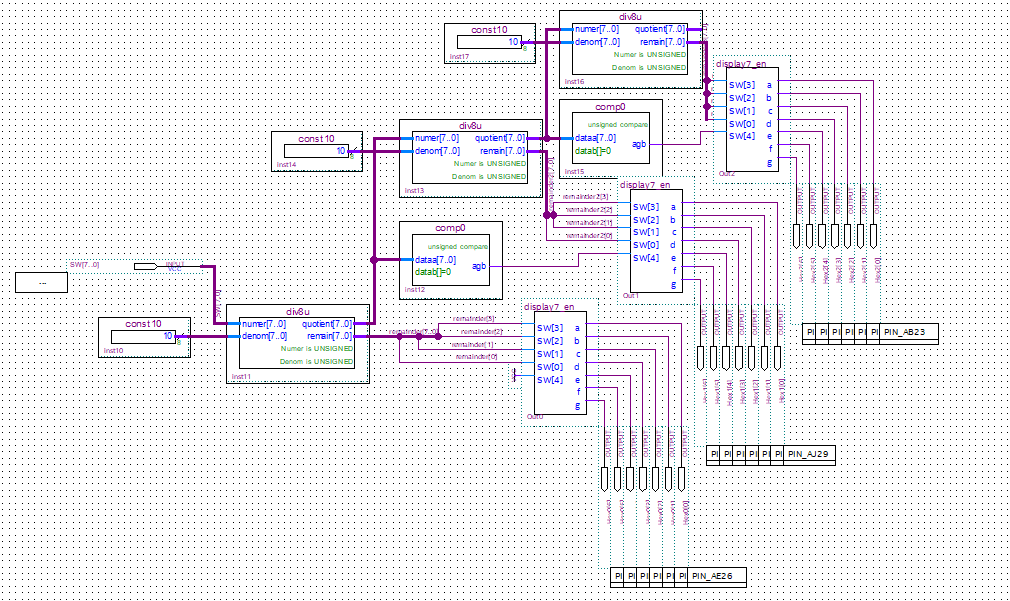
\includegraphics[width=.9\textwidth]{Figures/8BDesign.png}
  \caption{8-Bit Unsigned Integer on 7-Segment Display Circuit}
  \label{fig:1}
\end{figure}

\hspace{.5 in} Unlike previous logic circuit verifications, this circuit was solely verified through uploading to the DE1-SoC board and changing the switches to provide different inputs. The results of the verification are shown in Figures \ref{fig:2}-\ref{fig:5}.

\begin{figure}[H]
  \centering
  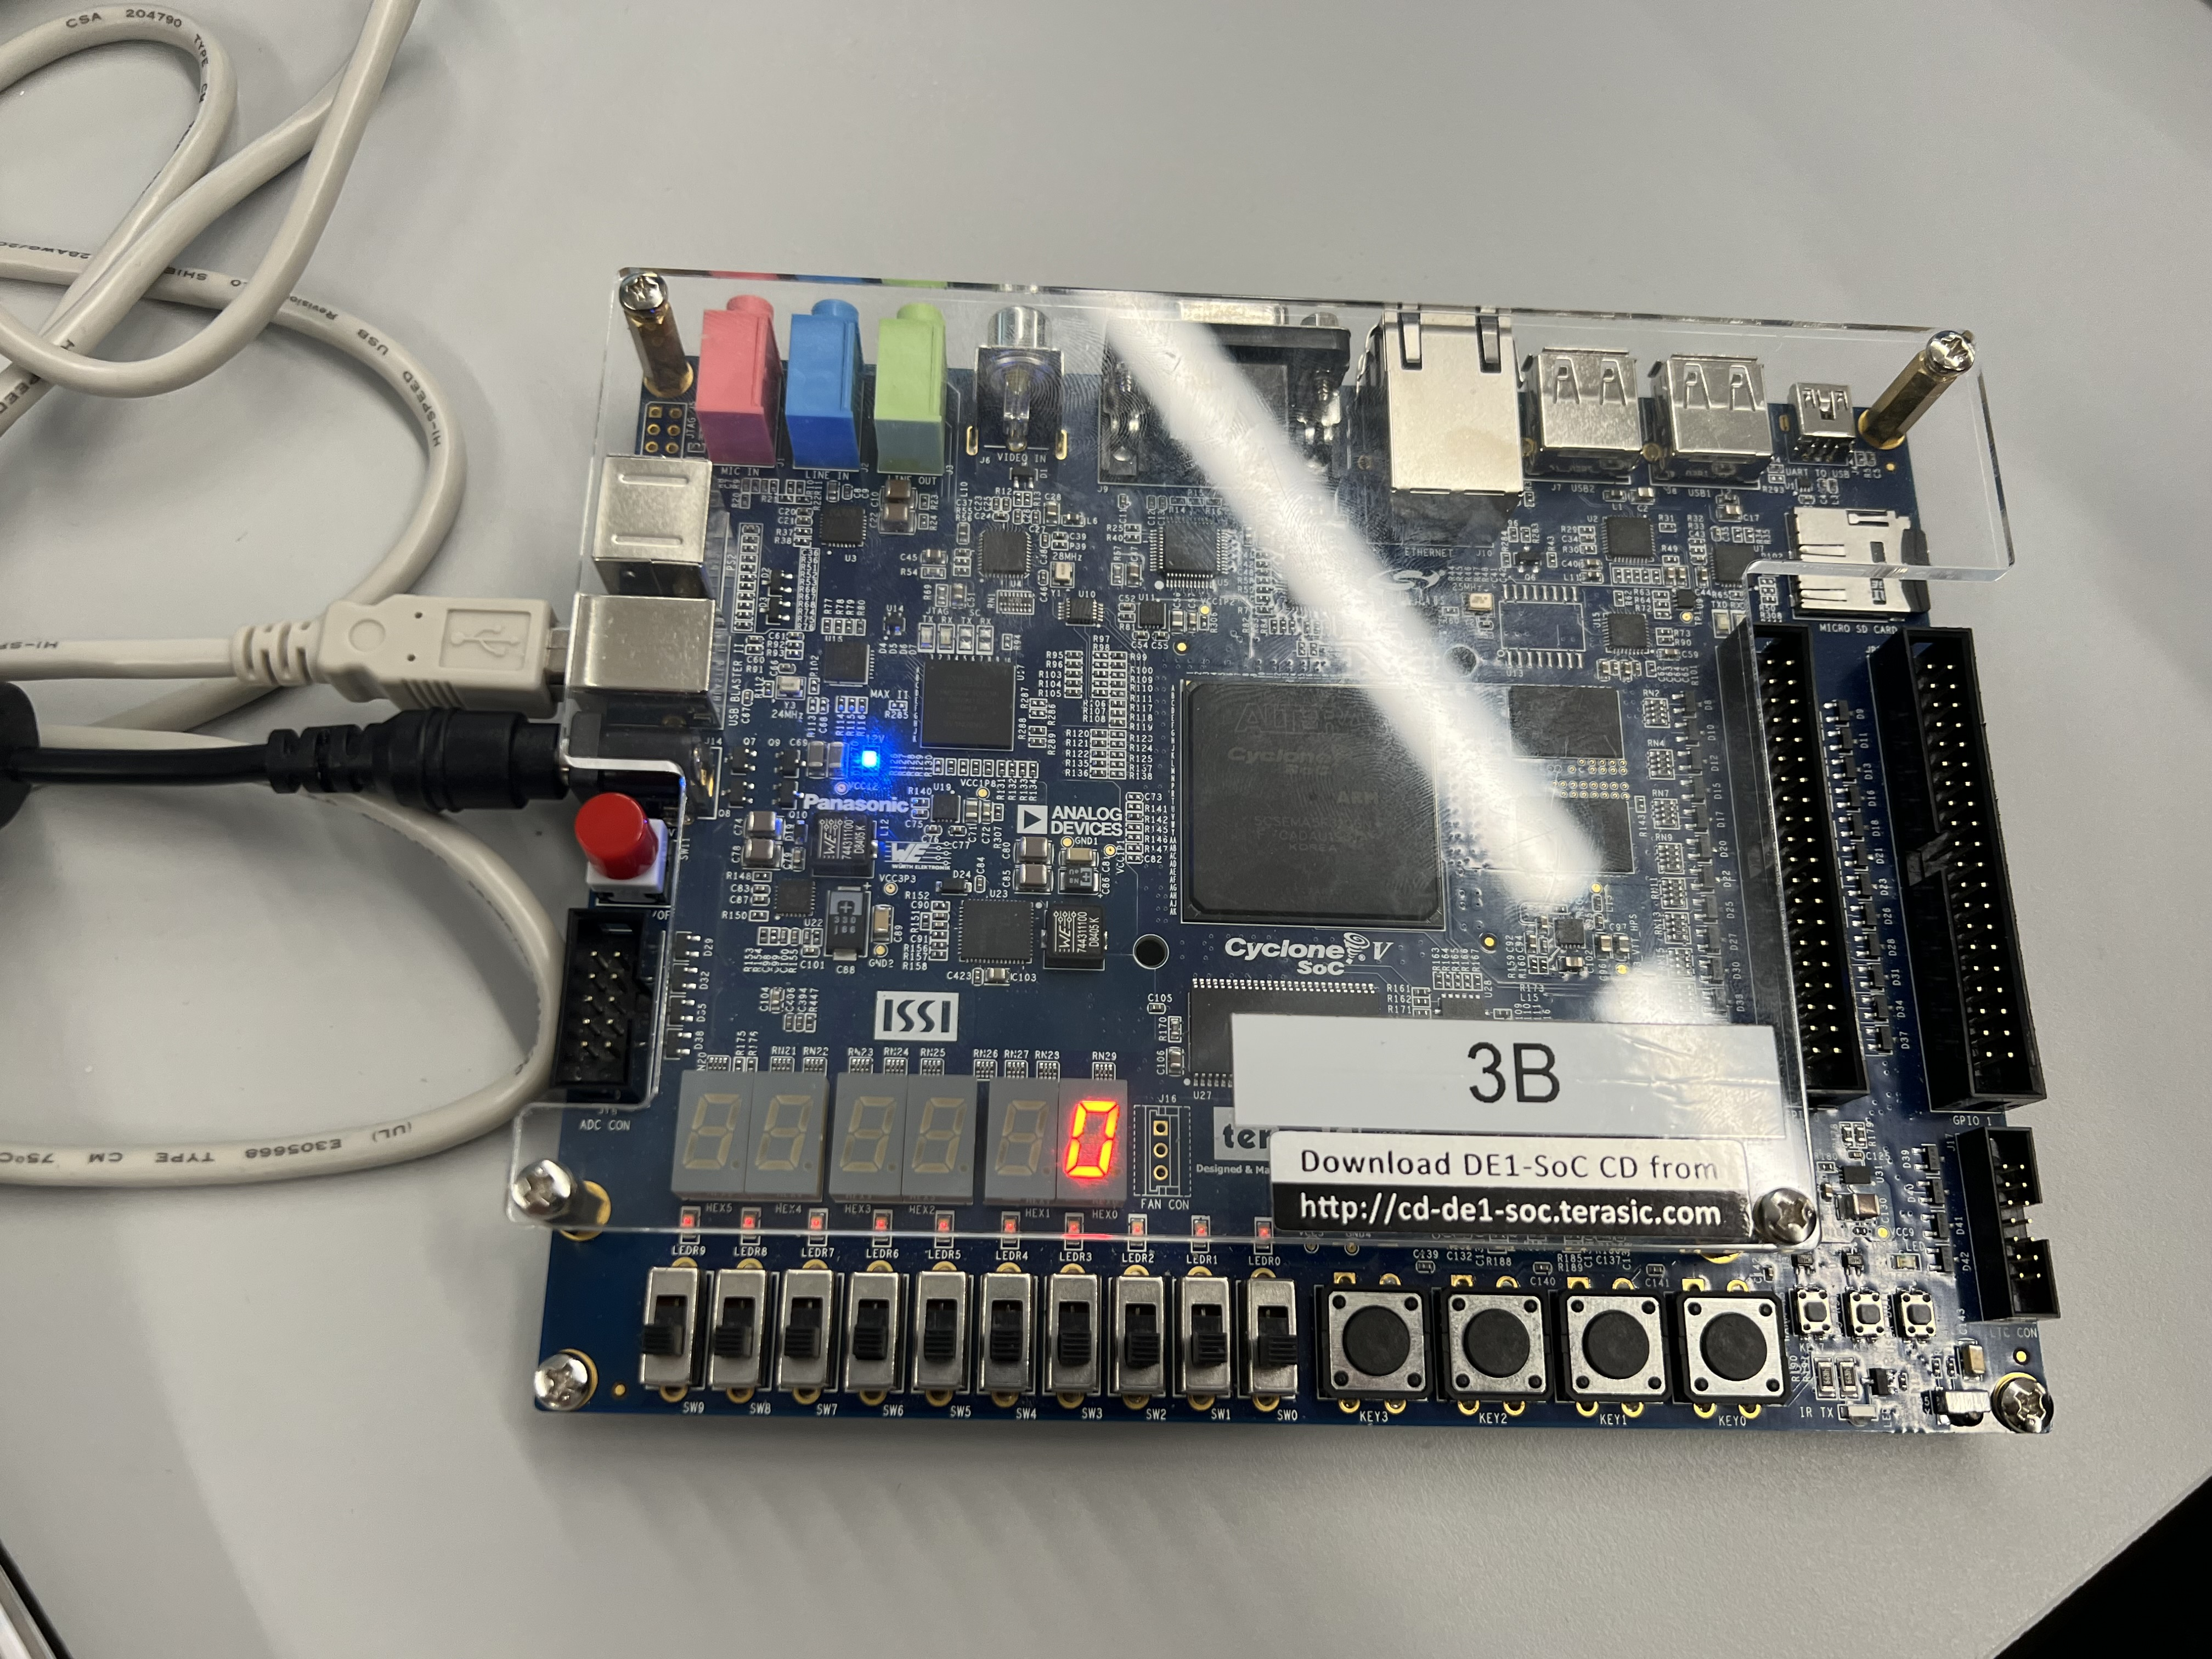
\includegraphics[width=.9\textwidth]{Figures/Part\ 1/IMG_1074.jpg}
  \caption{$00000000_2$ Input on Switches, Displaying $0$}
  \label{fig:2}
\end{figure}

\begin{figure}[H]
  \centering
  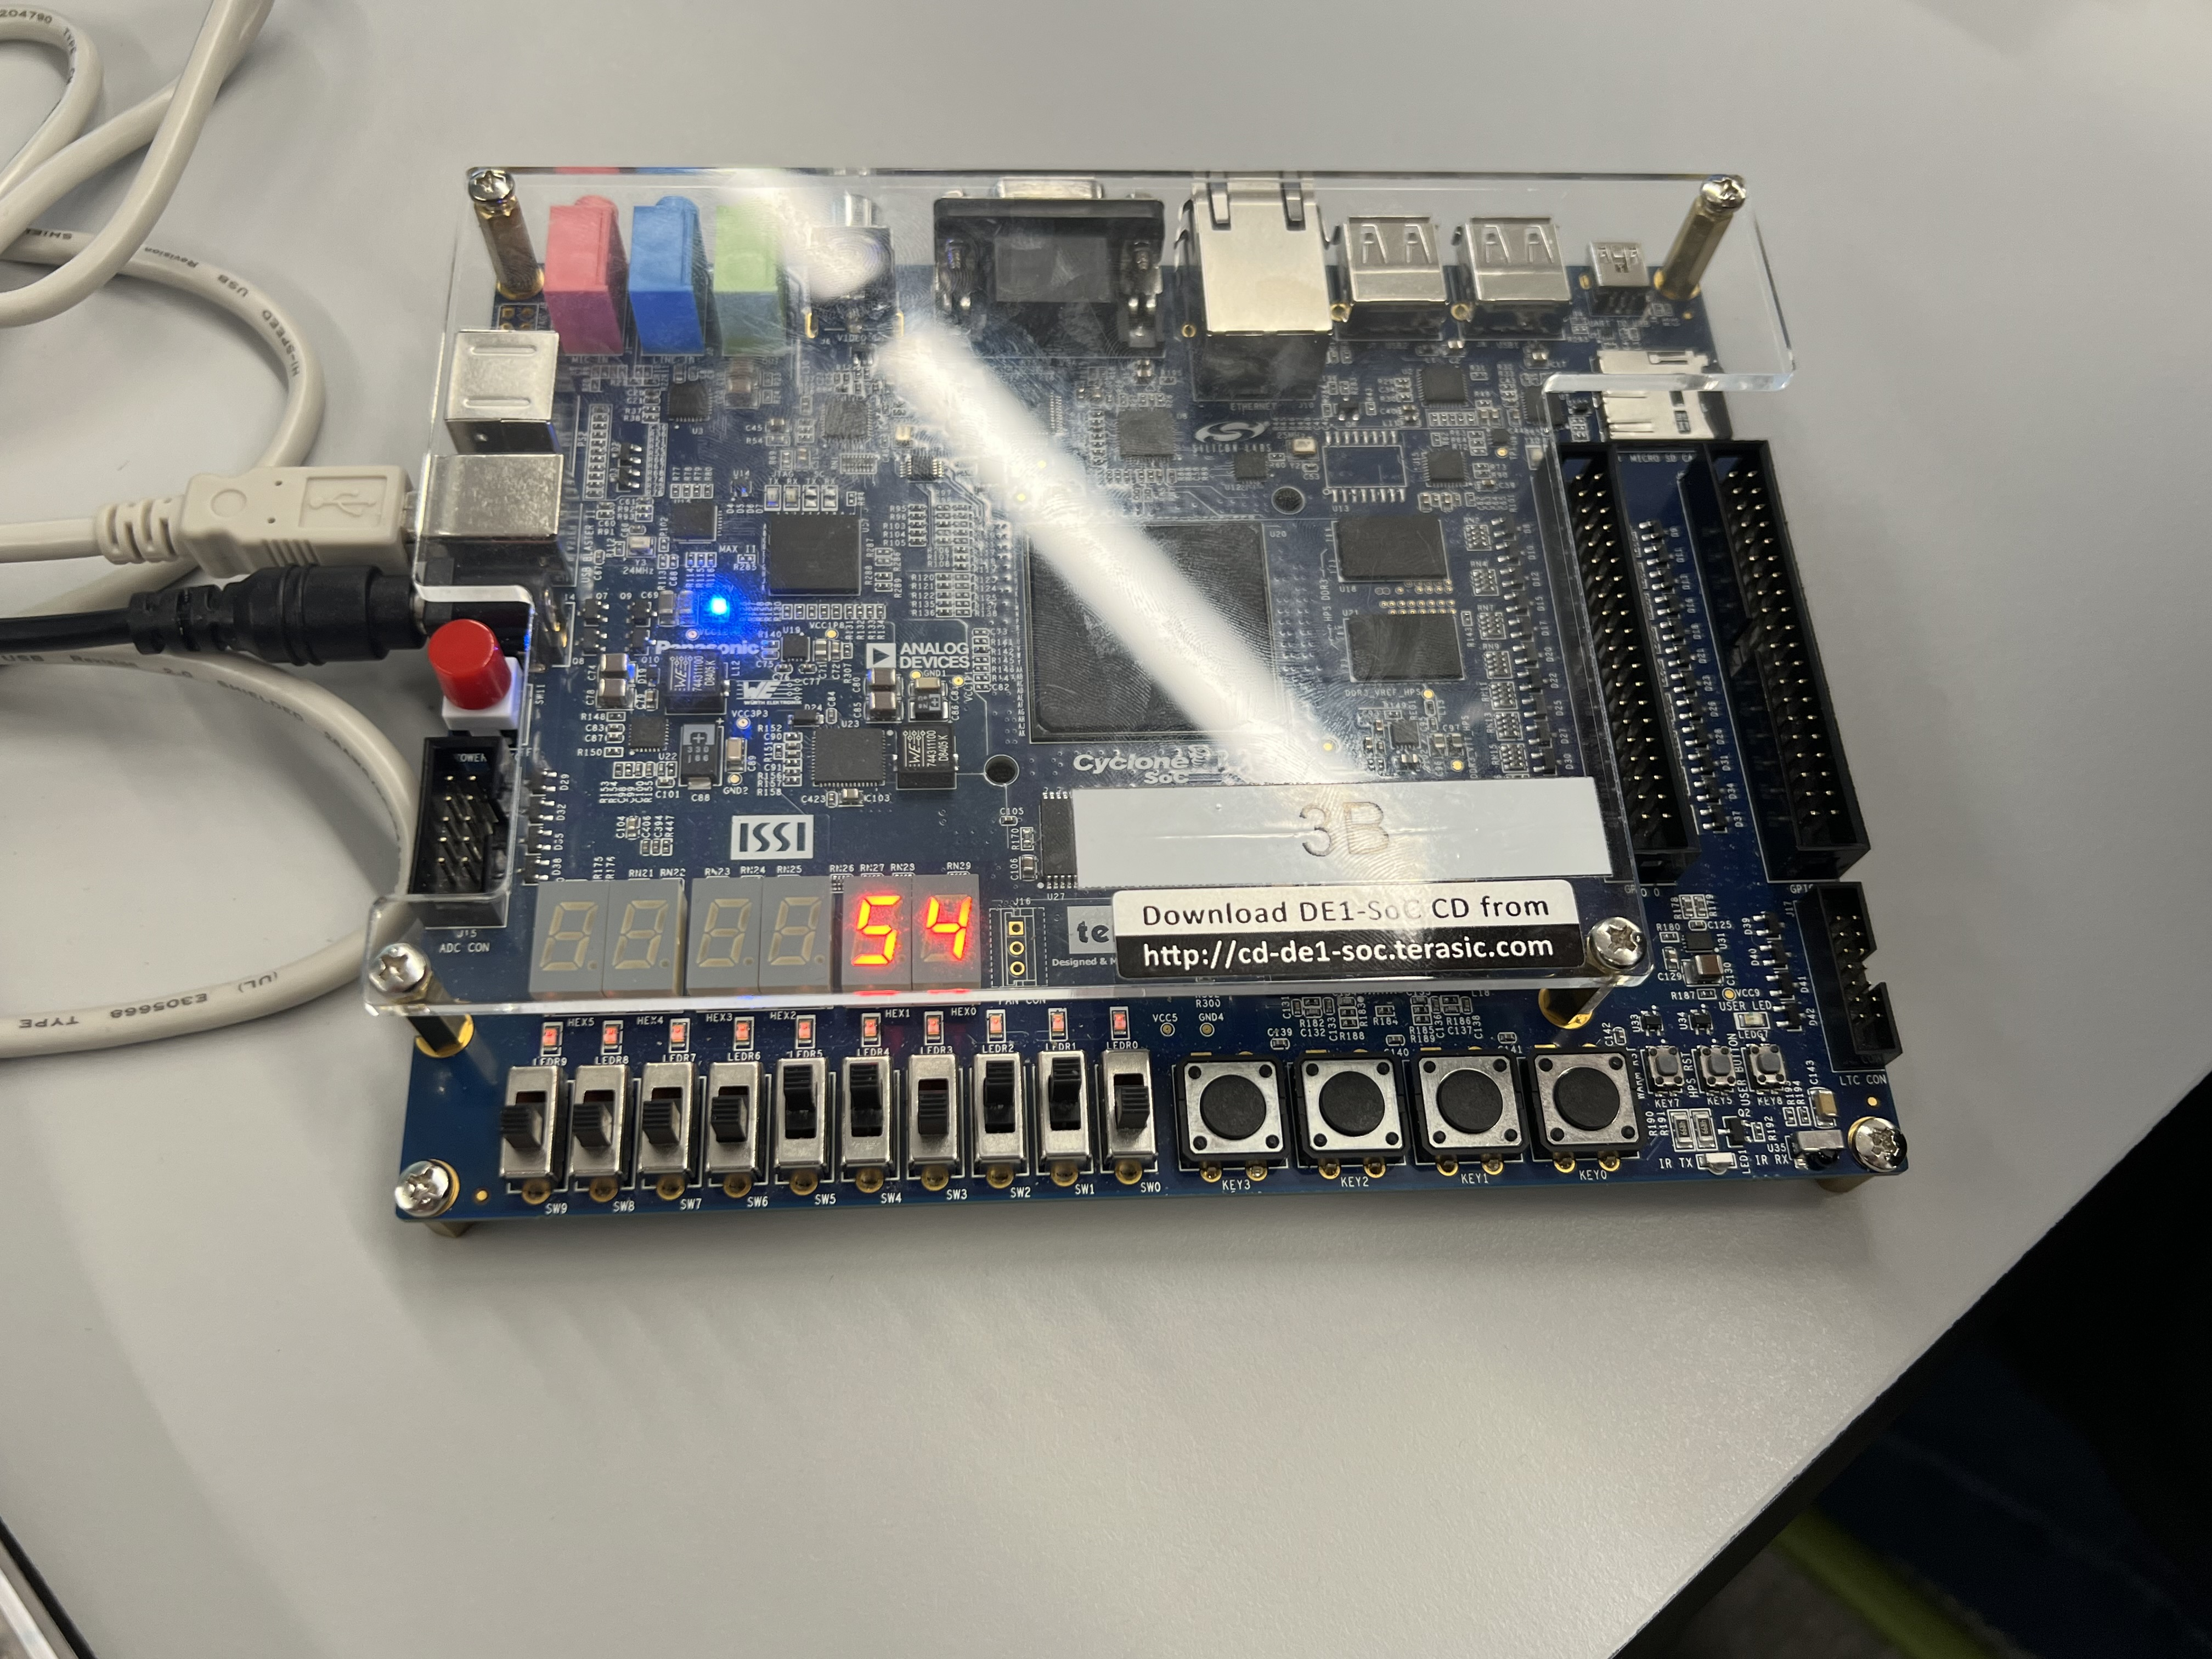
\includegraphics[width=.9\textwidth]{Figures/Part\ 1/IMG_1075.jpg}
  \caption{$00110110_2$ on the Switches, Displaying $54$}
  \label{fig:3}
\end{figure}

\begin{figure}[H]
  \centering
  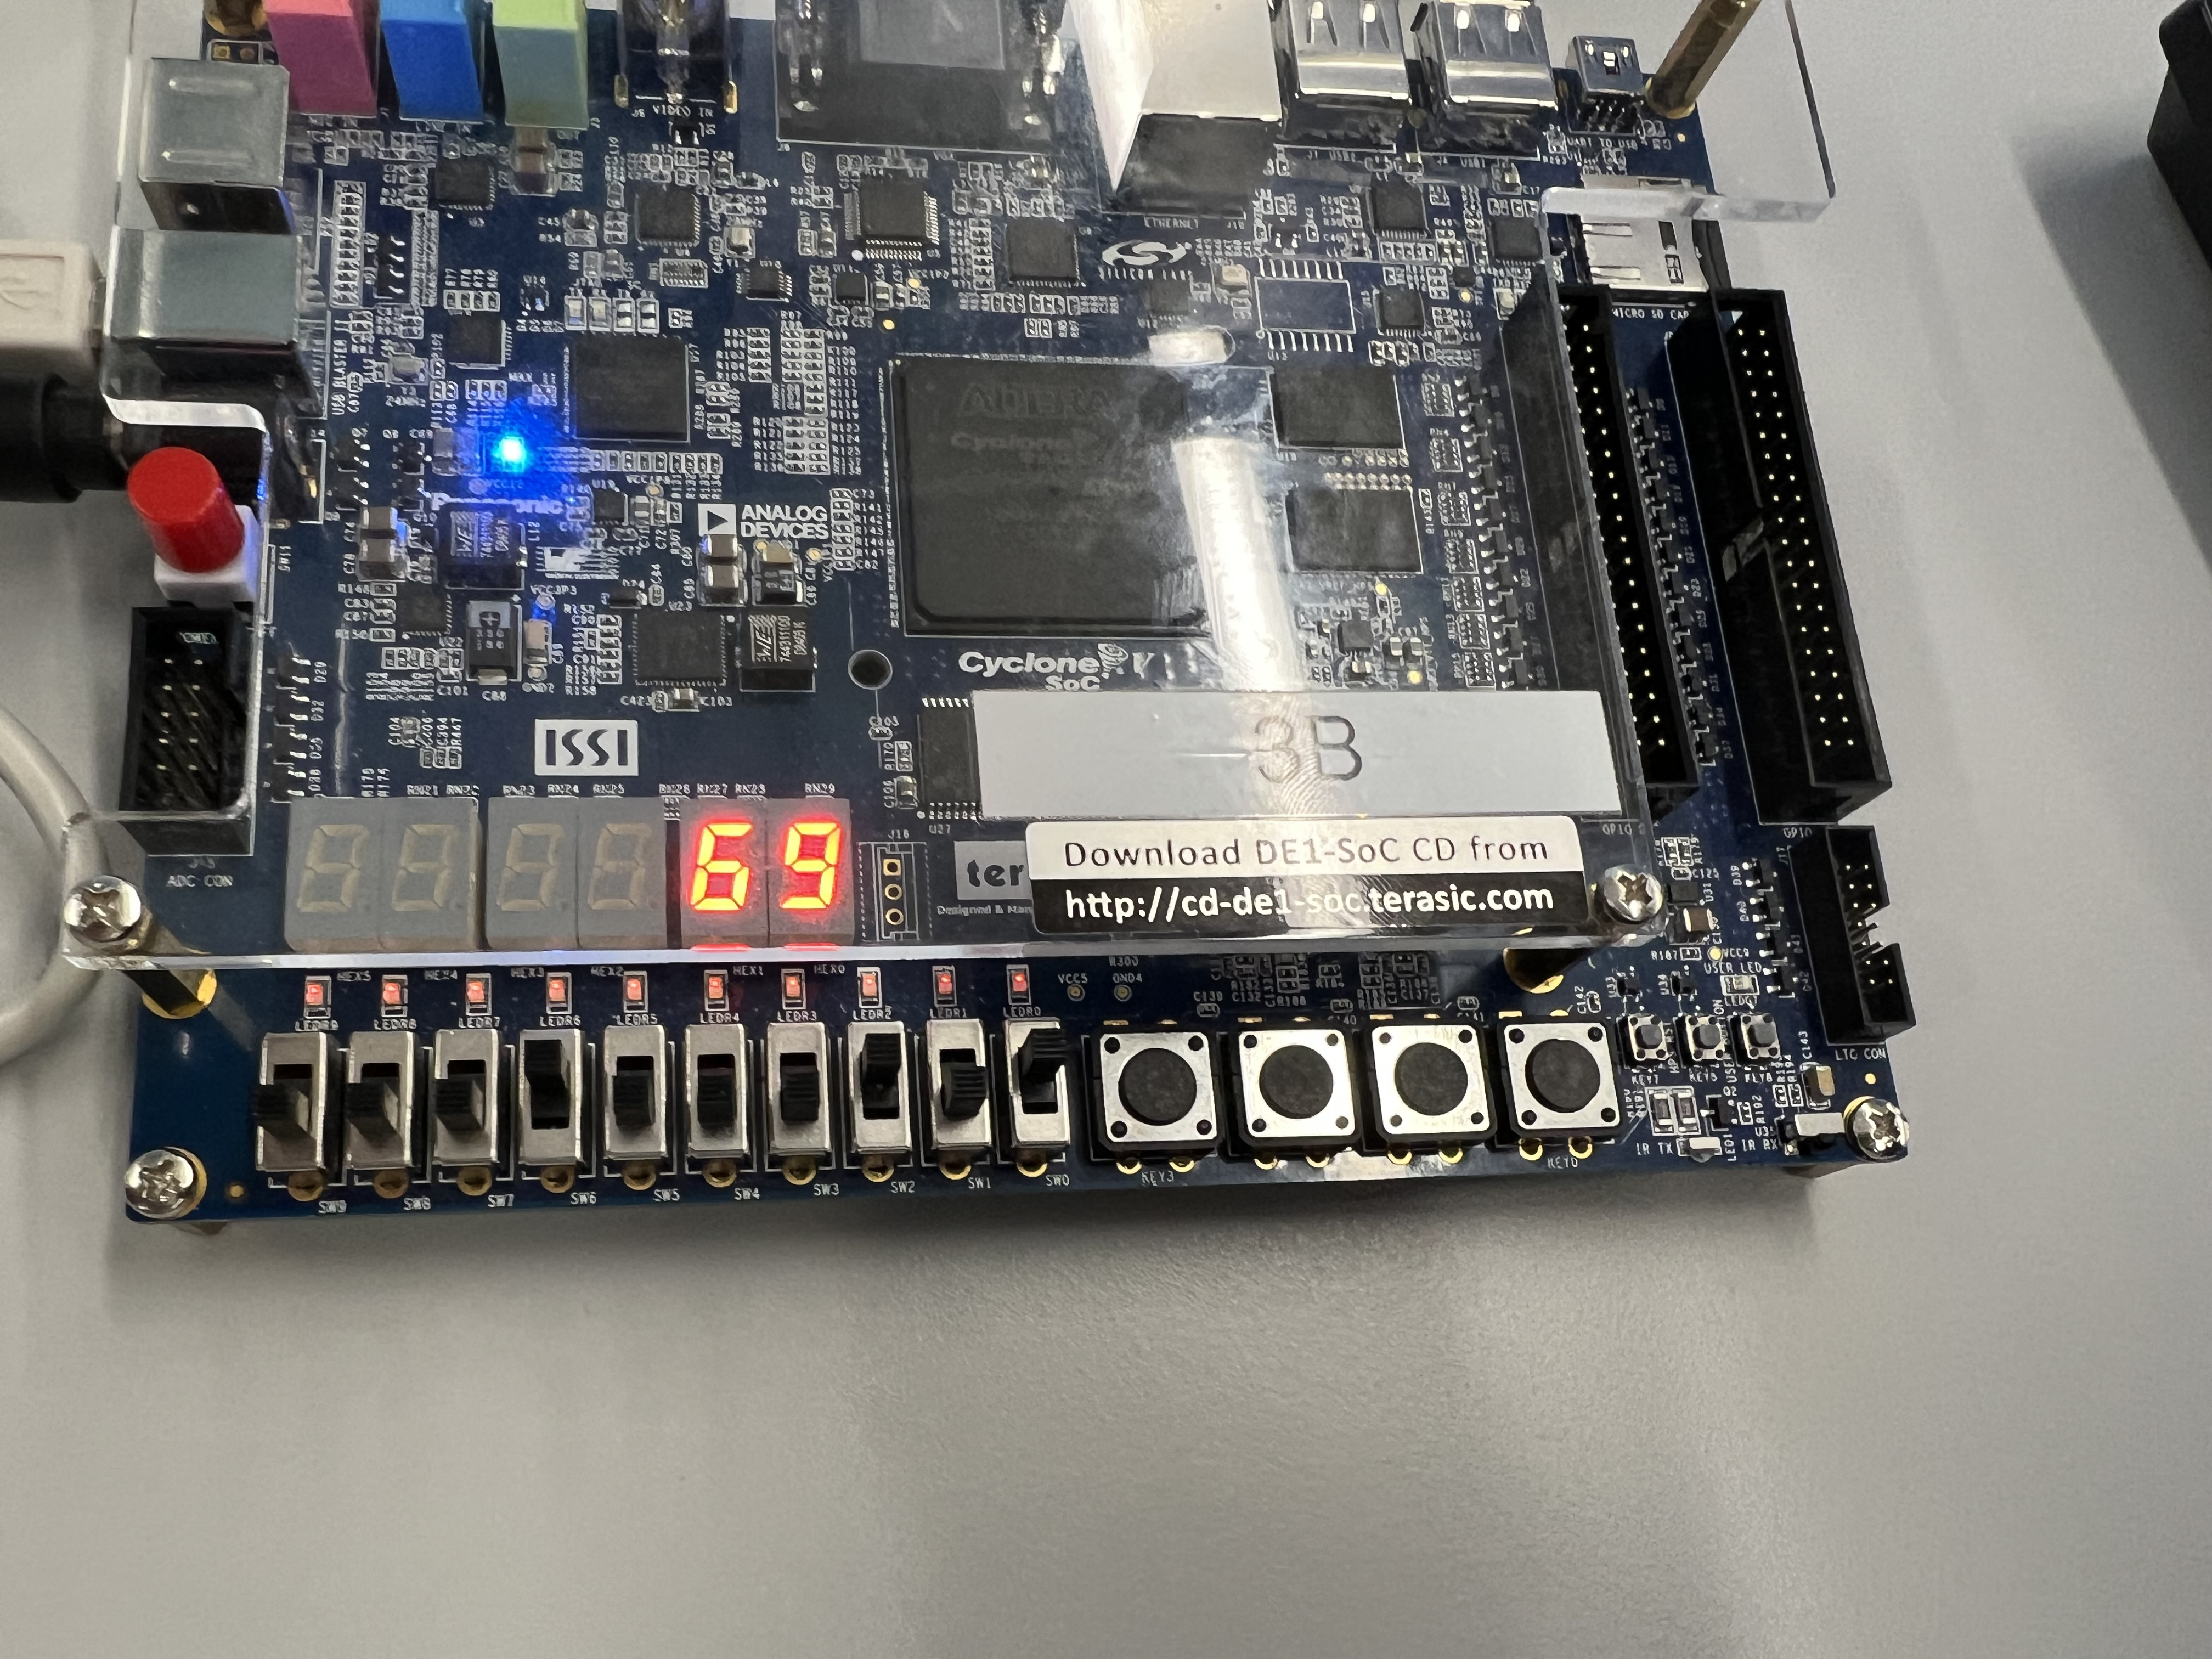
\includegraphics[width=.9\textwidth]{Figures/Part\ 1/IMG_1071.jpg}
  \caption{$01000101_2$ on the Switches, Displaying $69$}
  \label{fig:4}
\end{figure}

\begin{figure}[H]
  \centering
  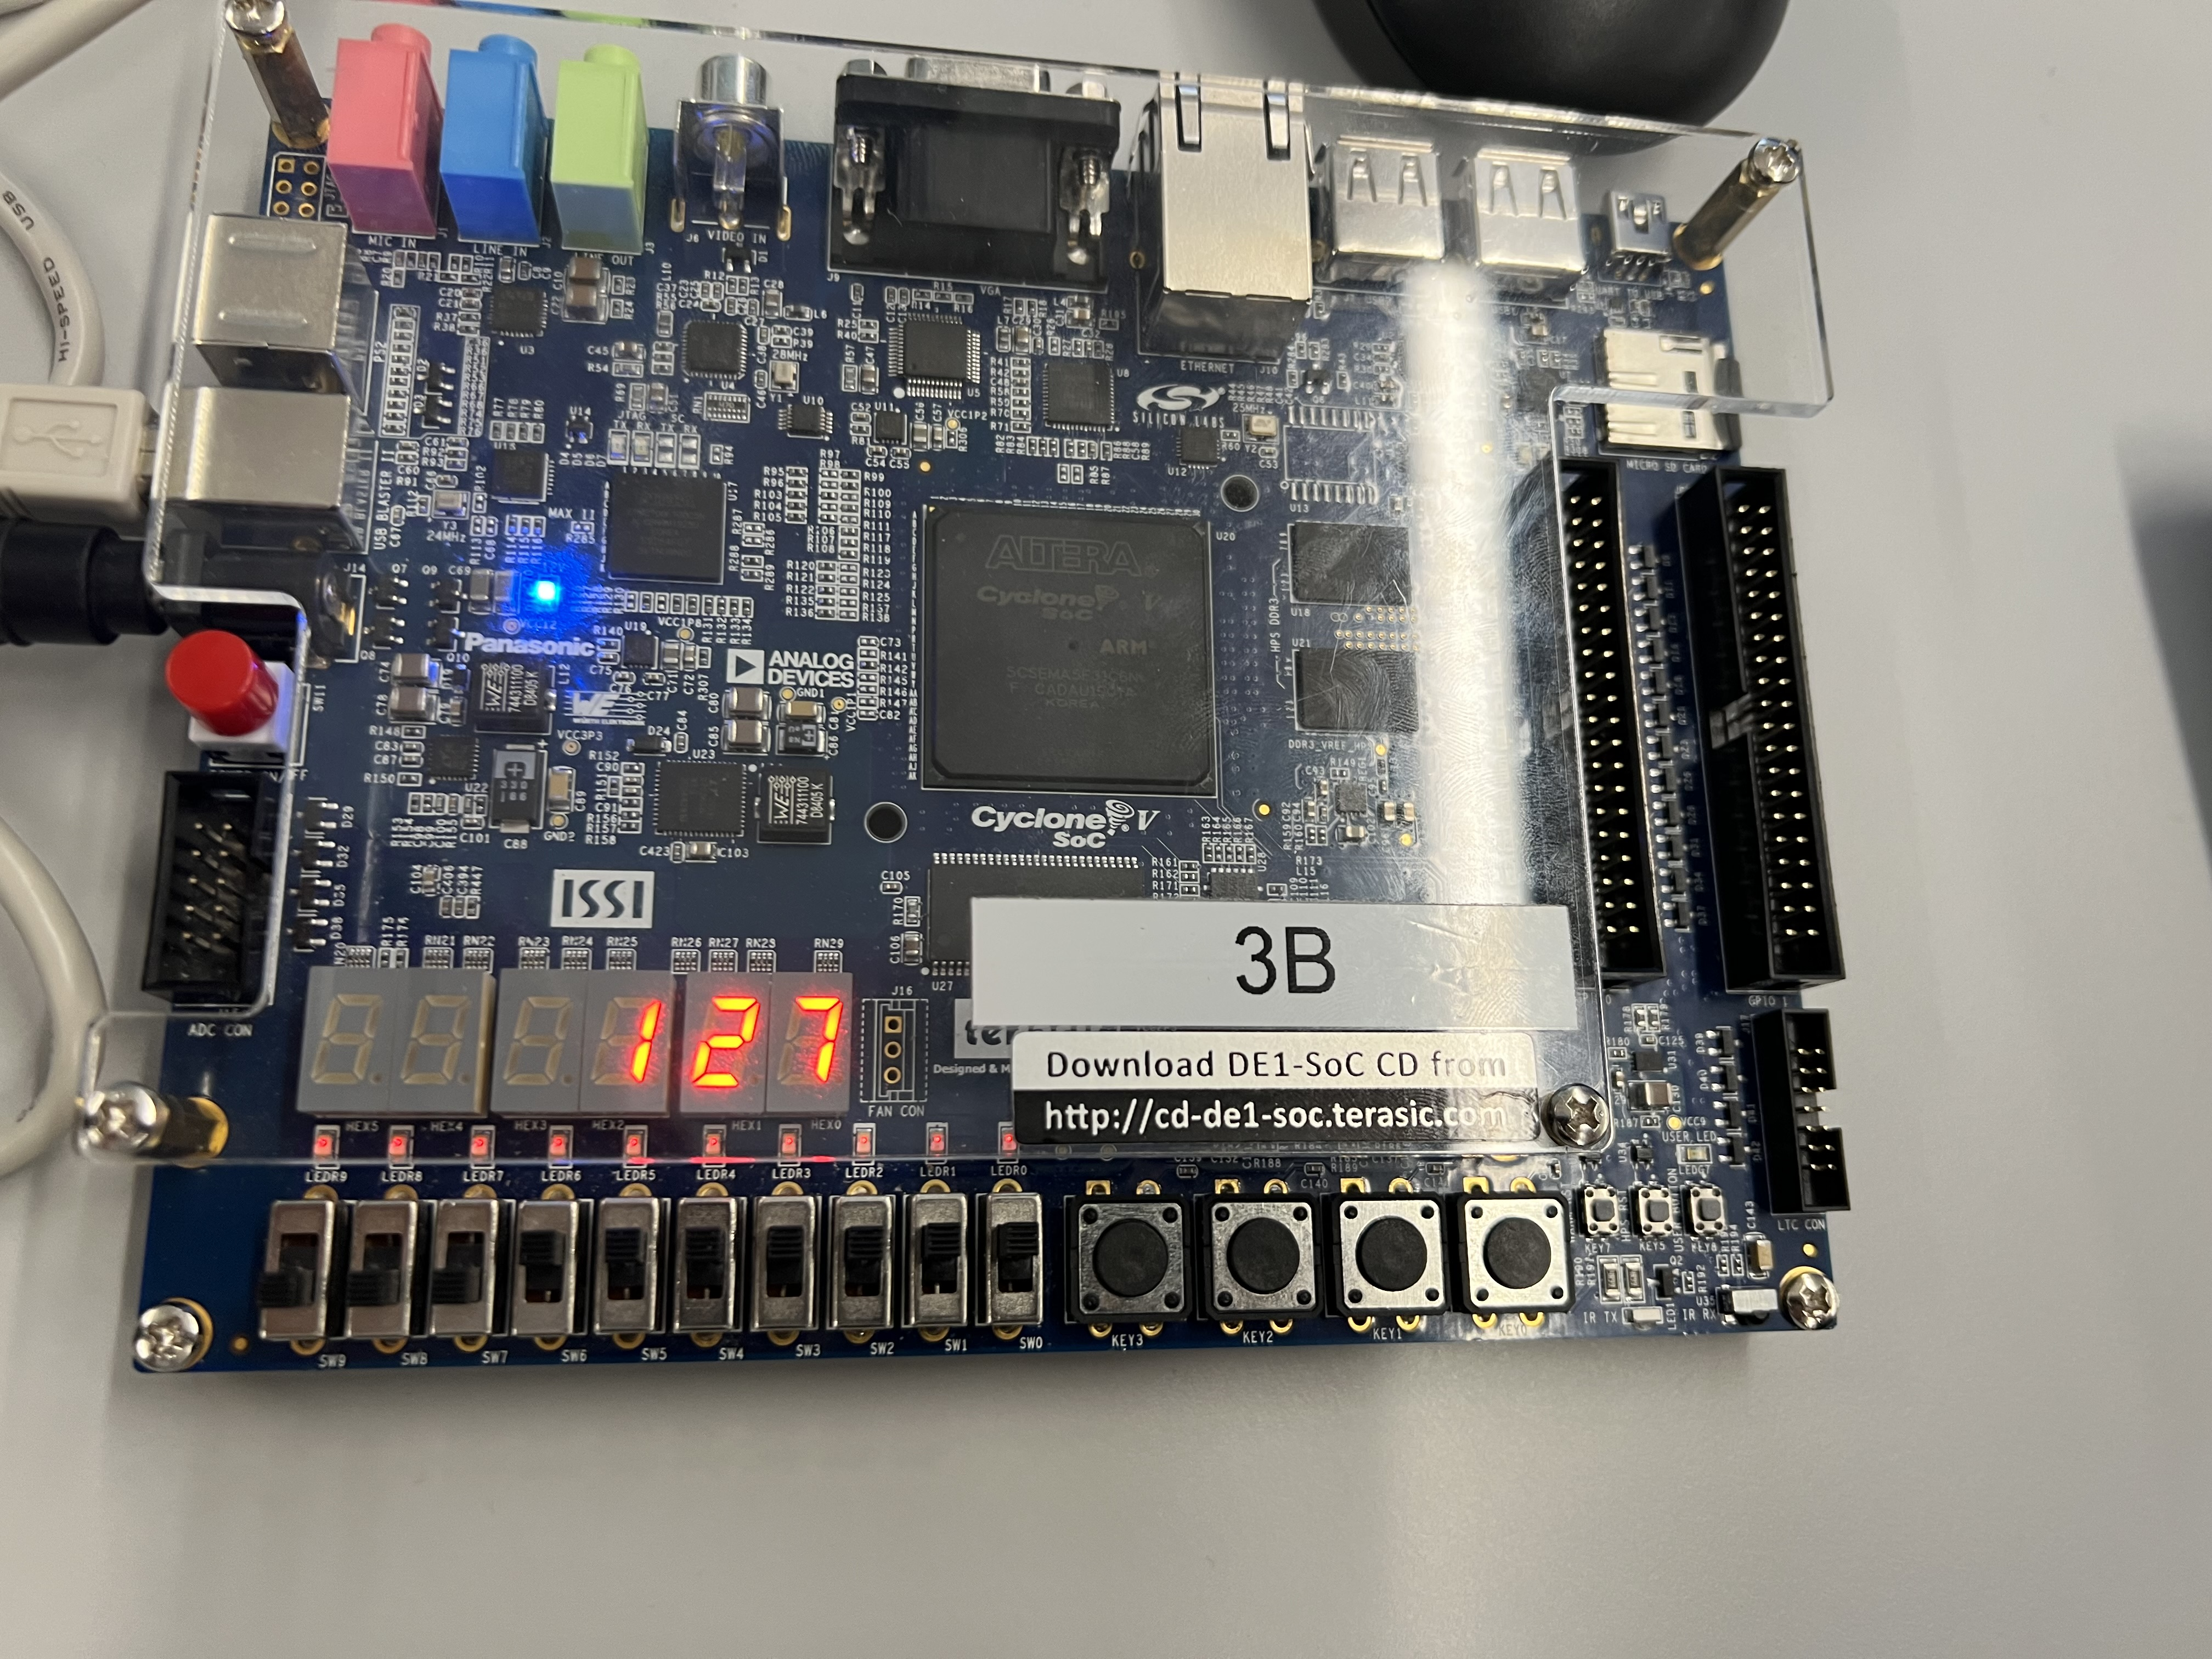
\includegraphics[width=.9\textwidth]{Figures/Part\ 1/IMG_1072.jpg}
  \caption{$01111111_2$ on Switches Displaying $127$}
  \label{fig:5}
\end{figure}

\subsection{Assignment 2}

\hspace{.5 in} The purpose of Assignment 2 was to create the ALU logic circuit with LPM modules addition, subtraction, multiplication and division. Given that there are limited switches on the DE1-SoC board, one 8-bit number was inputted to each LPM module, using SW[7..0], along with a constant decimal integer of ‘32.’ The outputs from these LPM modules were then all fed into a single 8-bit 4 to 1 multiplexer, which served to indicate what operation was to be performed with the control inputs of SW[8] and SW[9]. For the code of the inputs, 00 designated addition, 01 designated subtraction, 10 designated multiplication and 11 designated division. The multiplexer then output an 8-bit binary, positive integer that needed to be displayed on both the 7-segment displays and the LEDs. For the 7-segment displays, the logic circuit from Assignment 1 was used. The circuit was compressed into a function block called display\_8bits and added after the multiplexer. As for the LEDs, each LED from 0-7 was assigned a bit. If a bit was 1 then the LED would be on, but if the bit was a 0 then the LED would be off. The aforementioned schematic can be seen in Figure 6. 

\begin{figure}[H]
  \centering
  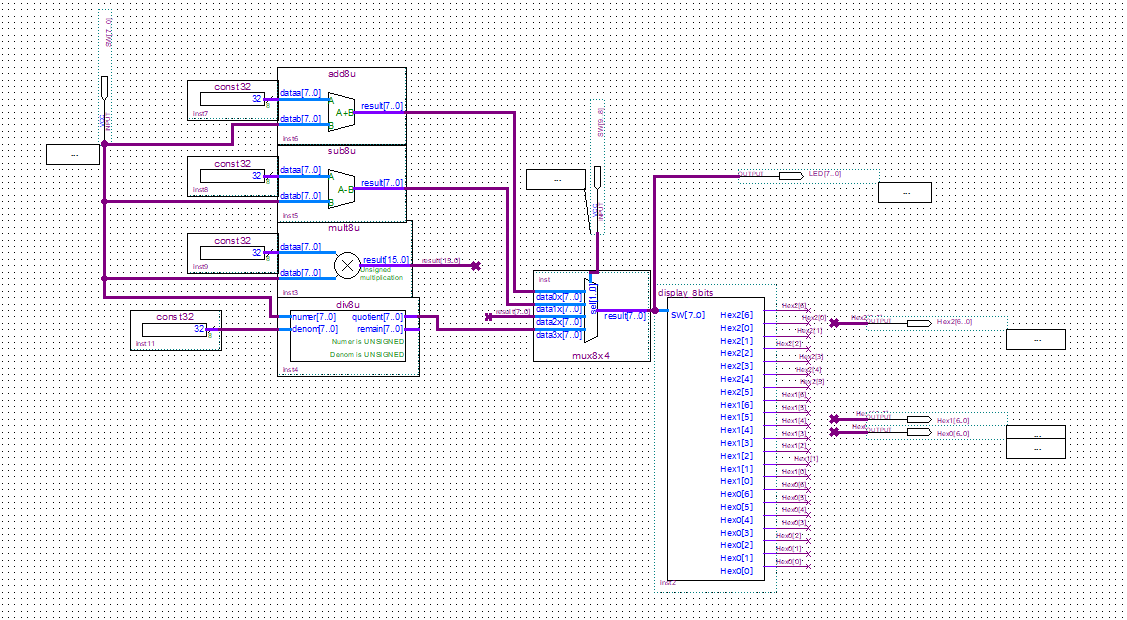
\includegraphics[width=.9\textwidth]{Figures/ALUDesign.png}
  \caption{ALU Design Schematic}
  \label{fig:6}
\end{figure}

\hspace{.5 in} Similar to Assignment 1, this logic circuit was not simulated in Waveform Simulation. The circuit was verified through uploading it to the board and testing different inputs. All operations were tested at least twice, and photos of the tests are shown in Figures \ref{fig:7}-\ref{fig:18} below.

\begin{figure}[H]
  \centering
  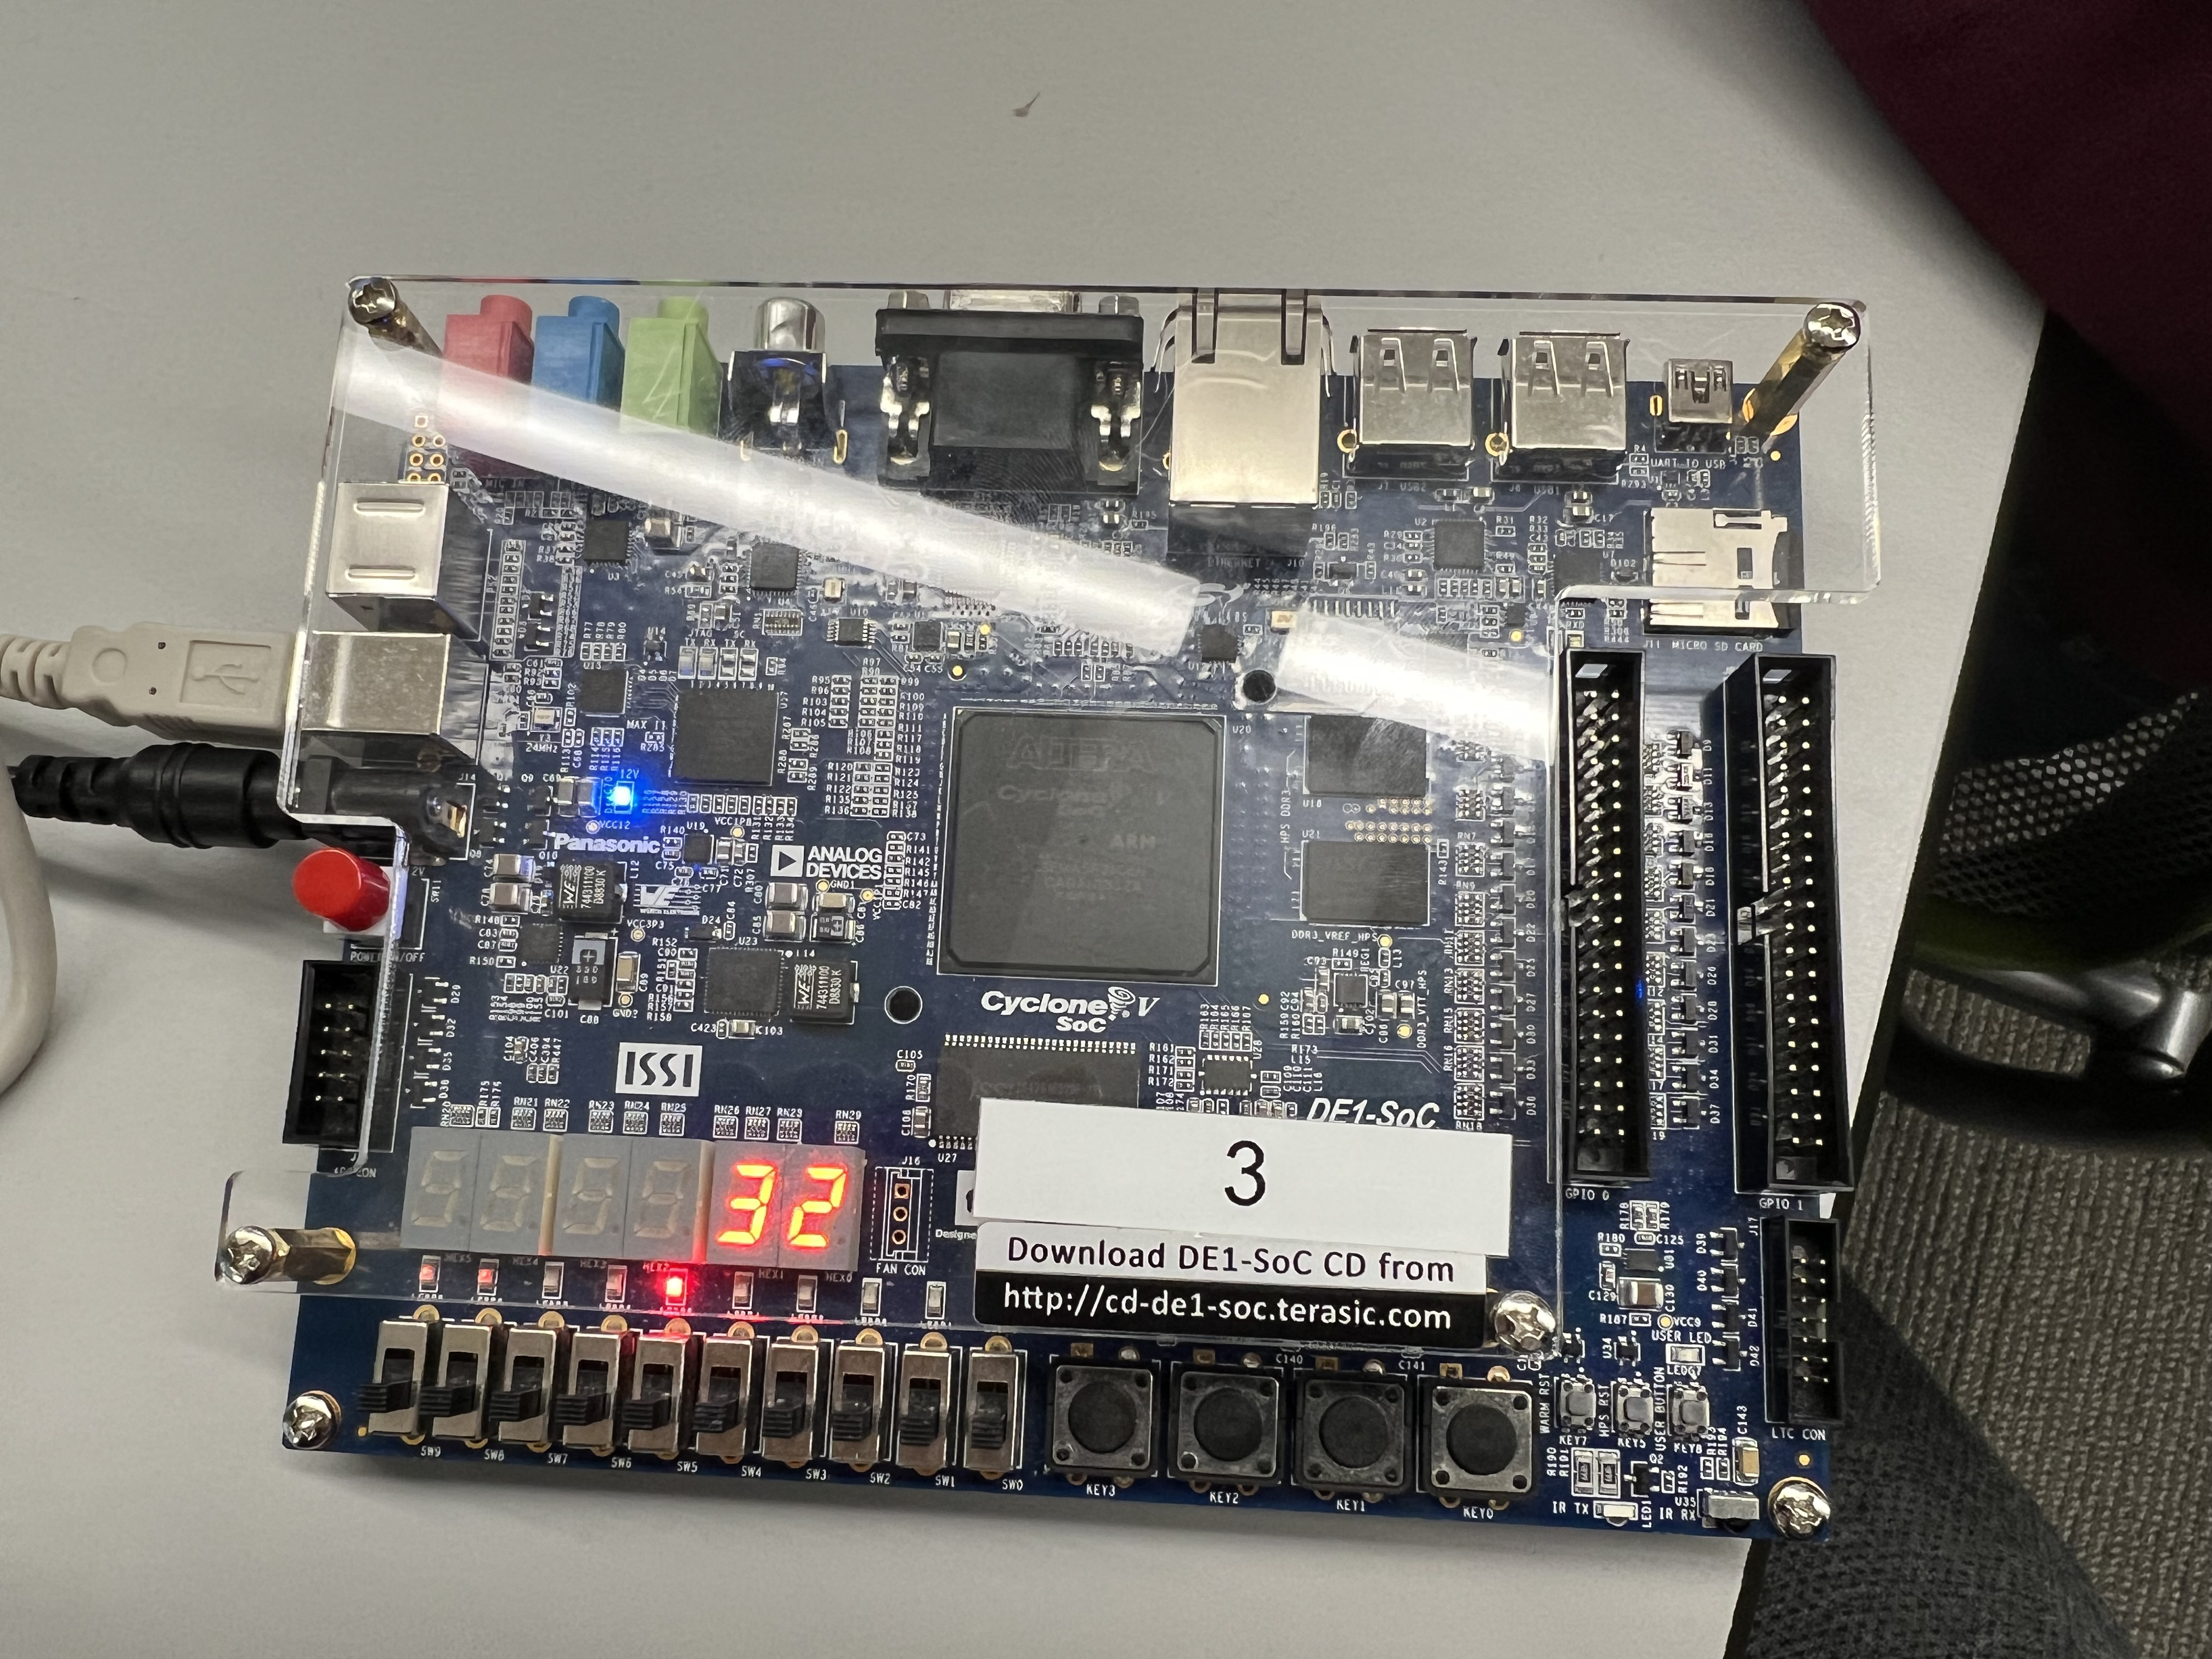
\includegraphics[width=.9\textwidth]{Figures/Part\ 2/IMG_1104.jpg}
  \caption{Addition — Constant $32$ and Binary Input of $00000000_2$ ($0$)}
  \label{fig:7}
\end{figure}

\begin{figure}[H]
  \centering
  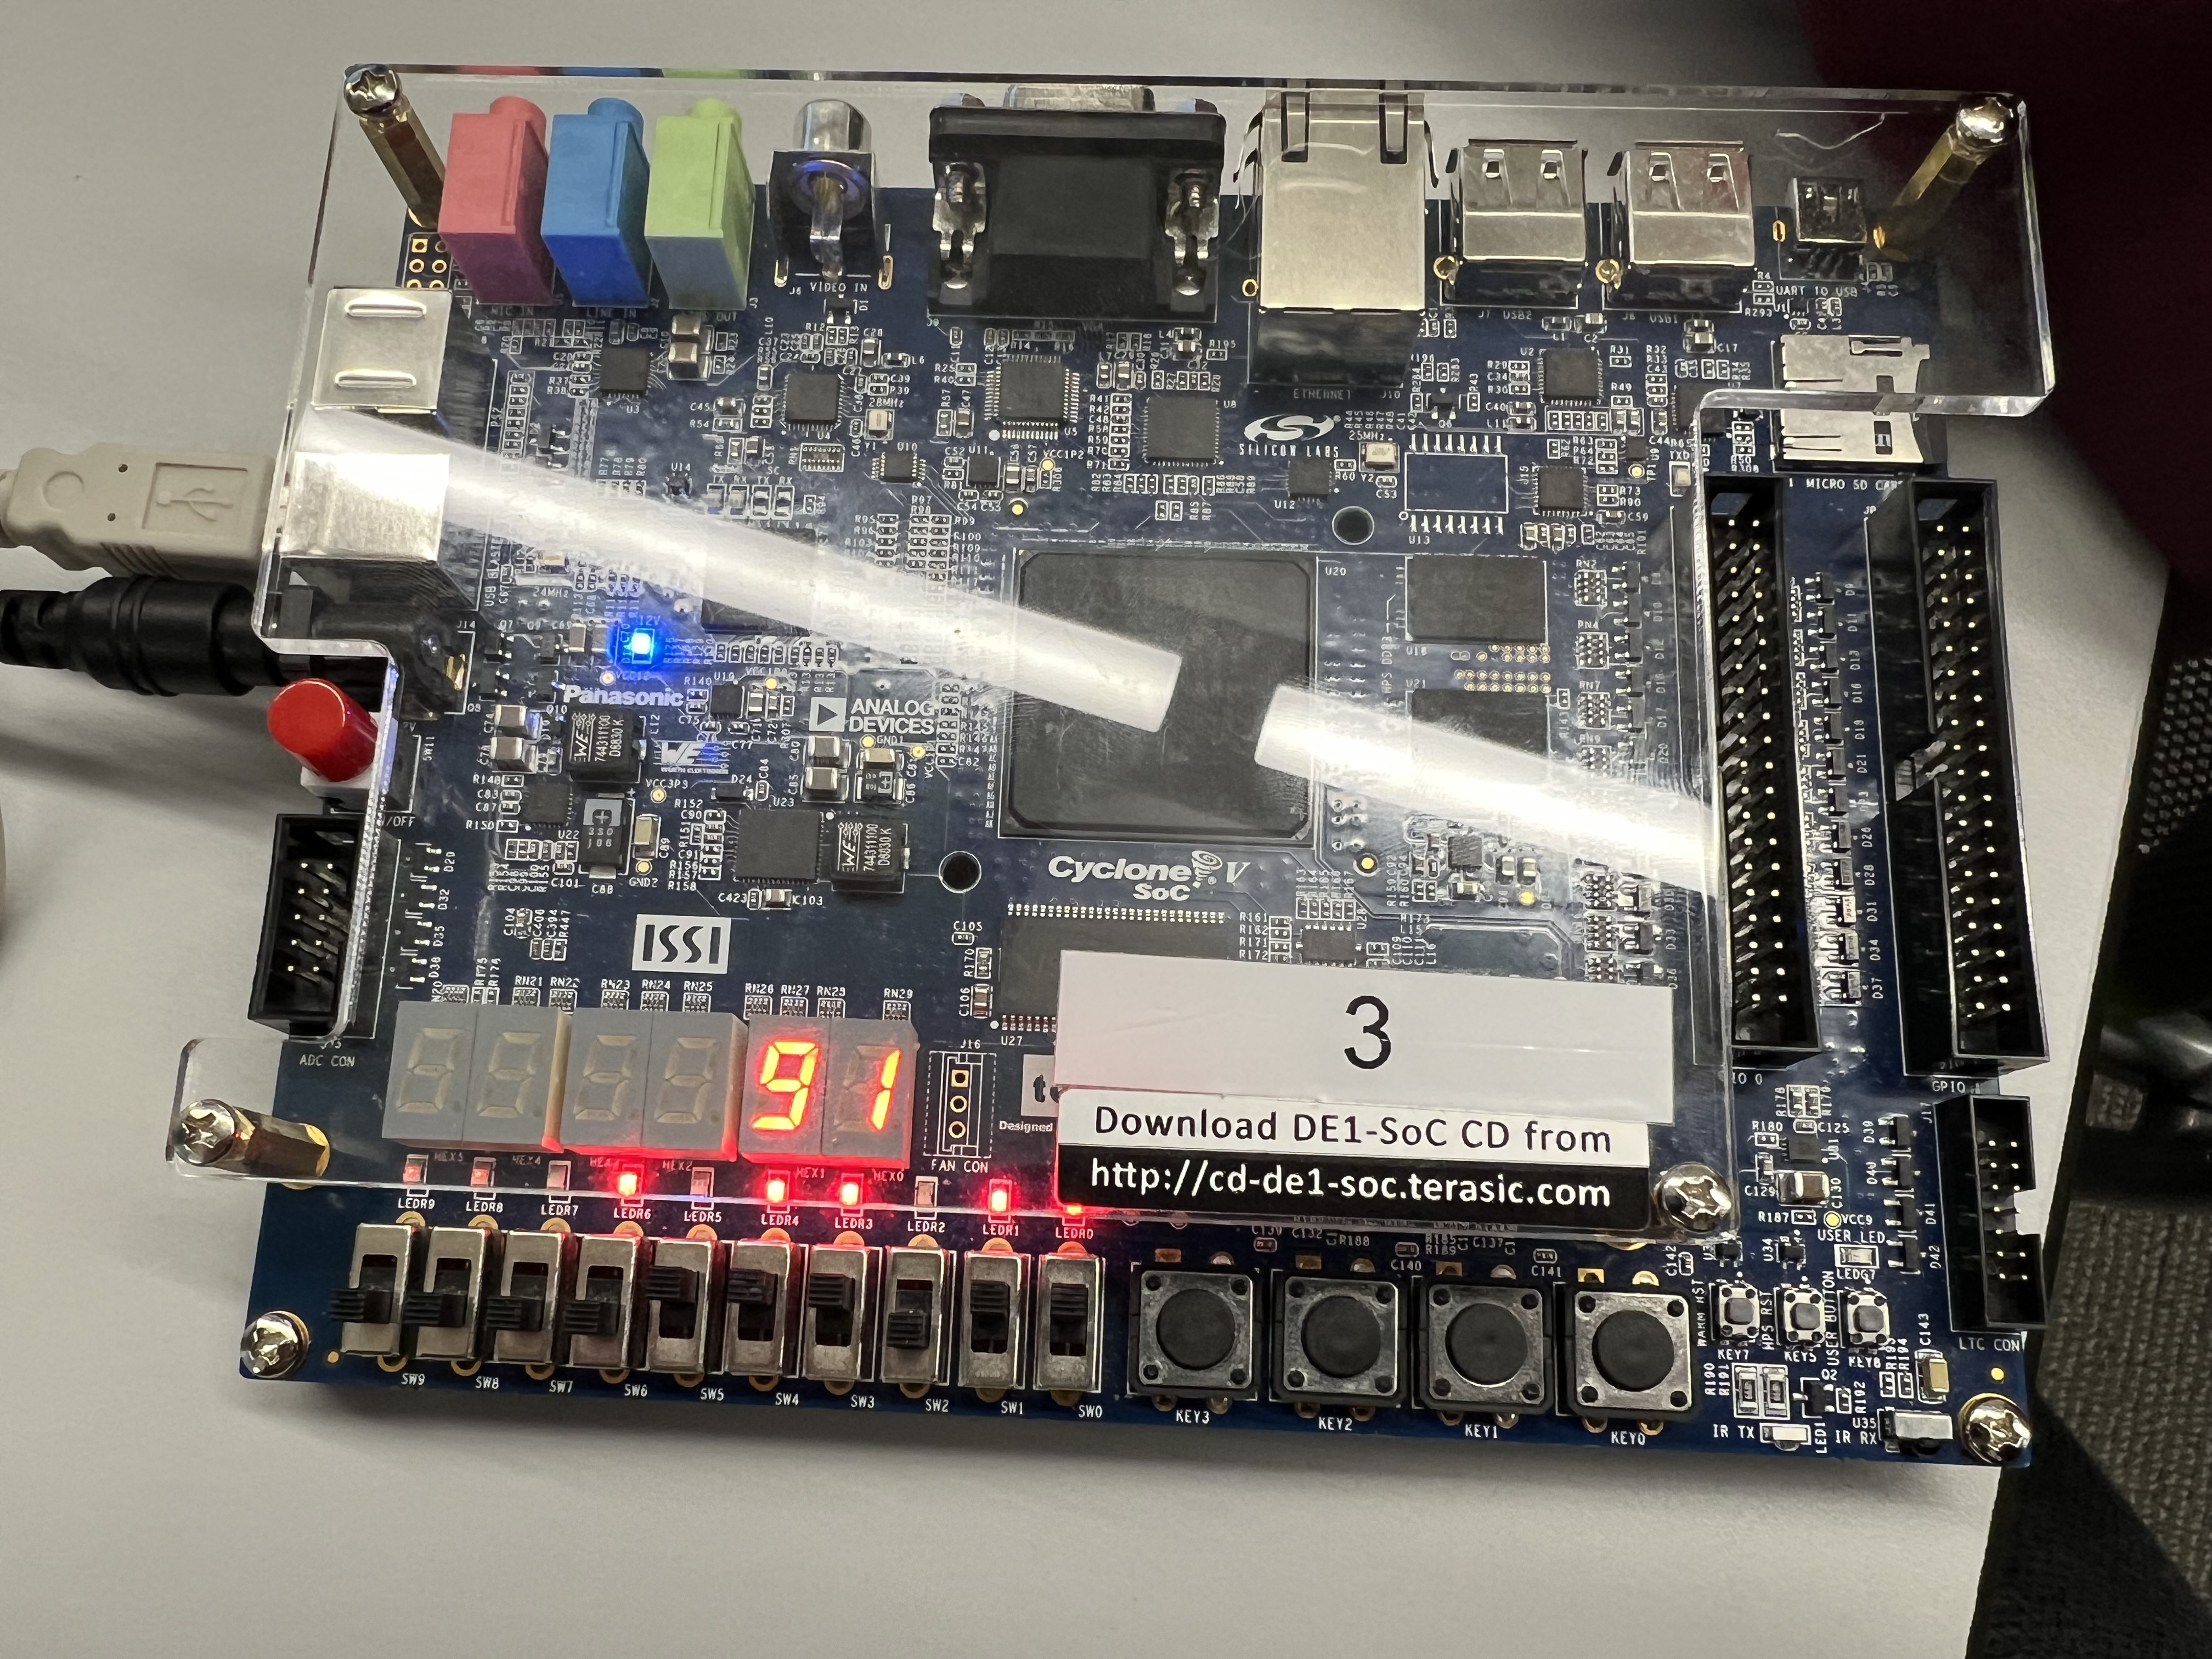
\includegraphics[width=.9\textwidth]{Figures/Part\ 2/IMG_1106.jpg}
  \caption{Addition — Constant $32$ and Binary Input of $00111011_2$ ($59$)}
  \label{fig:8}
\end{figure}

\begin{figure}[H]
  \centering
  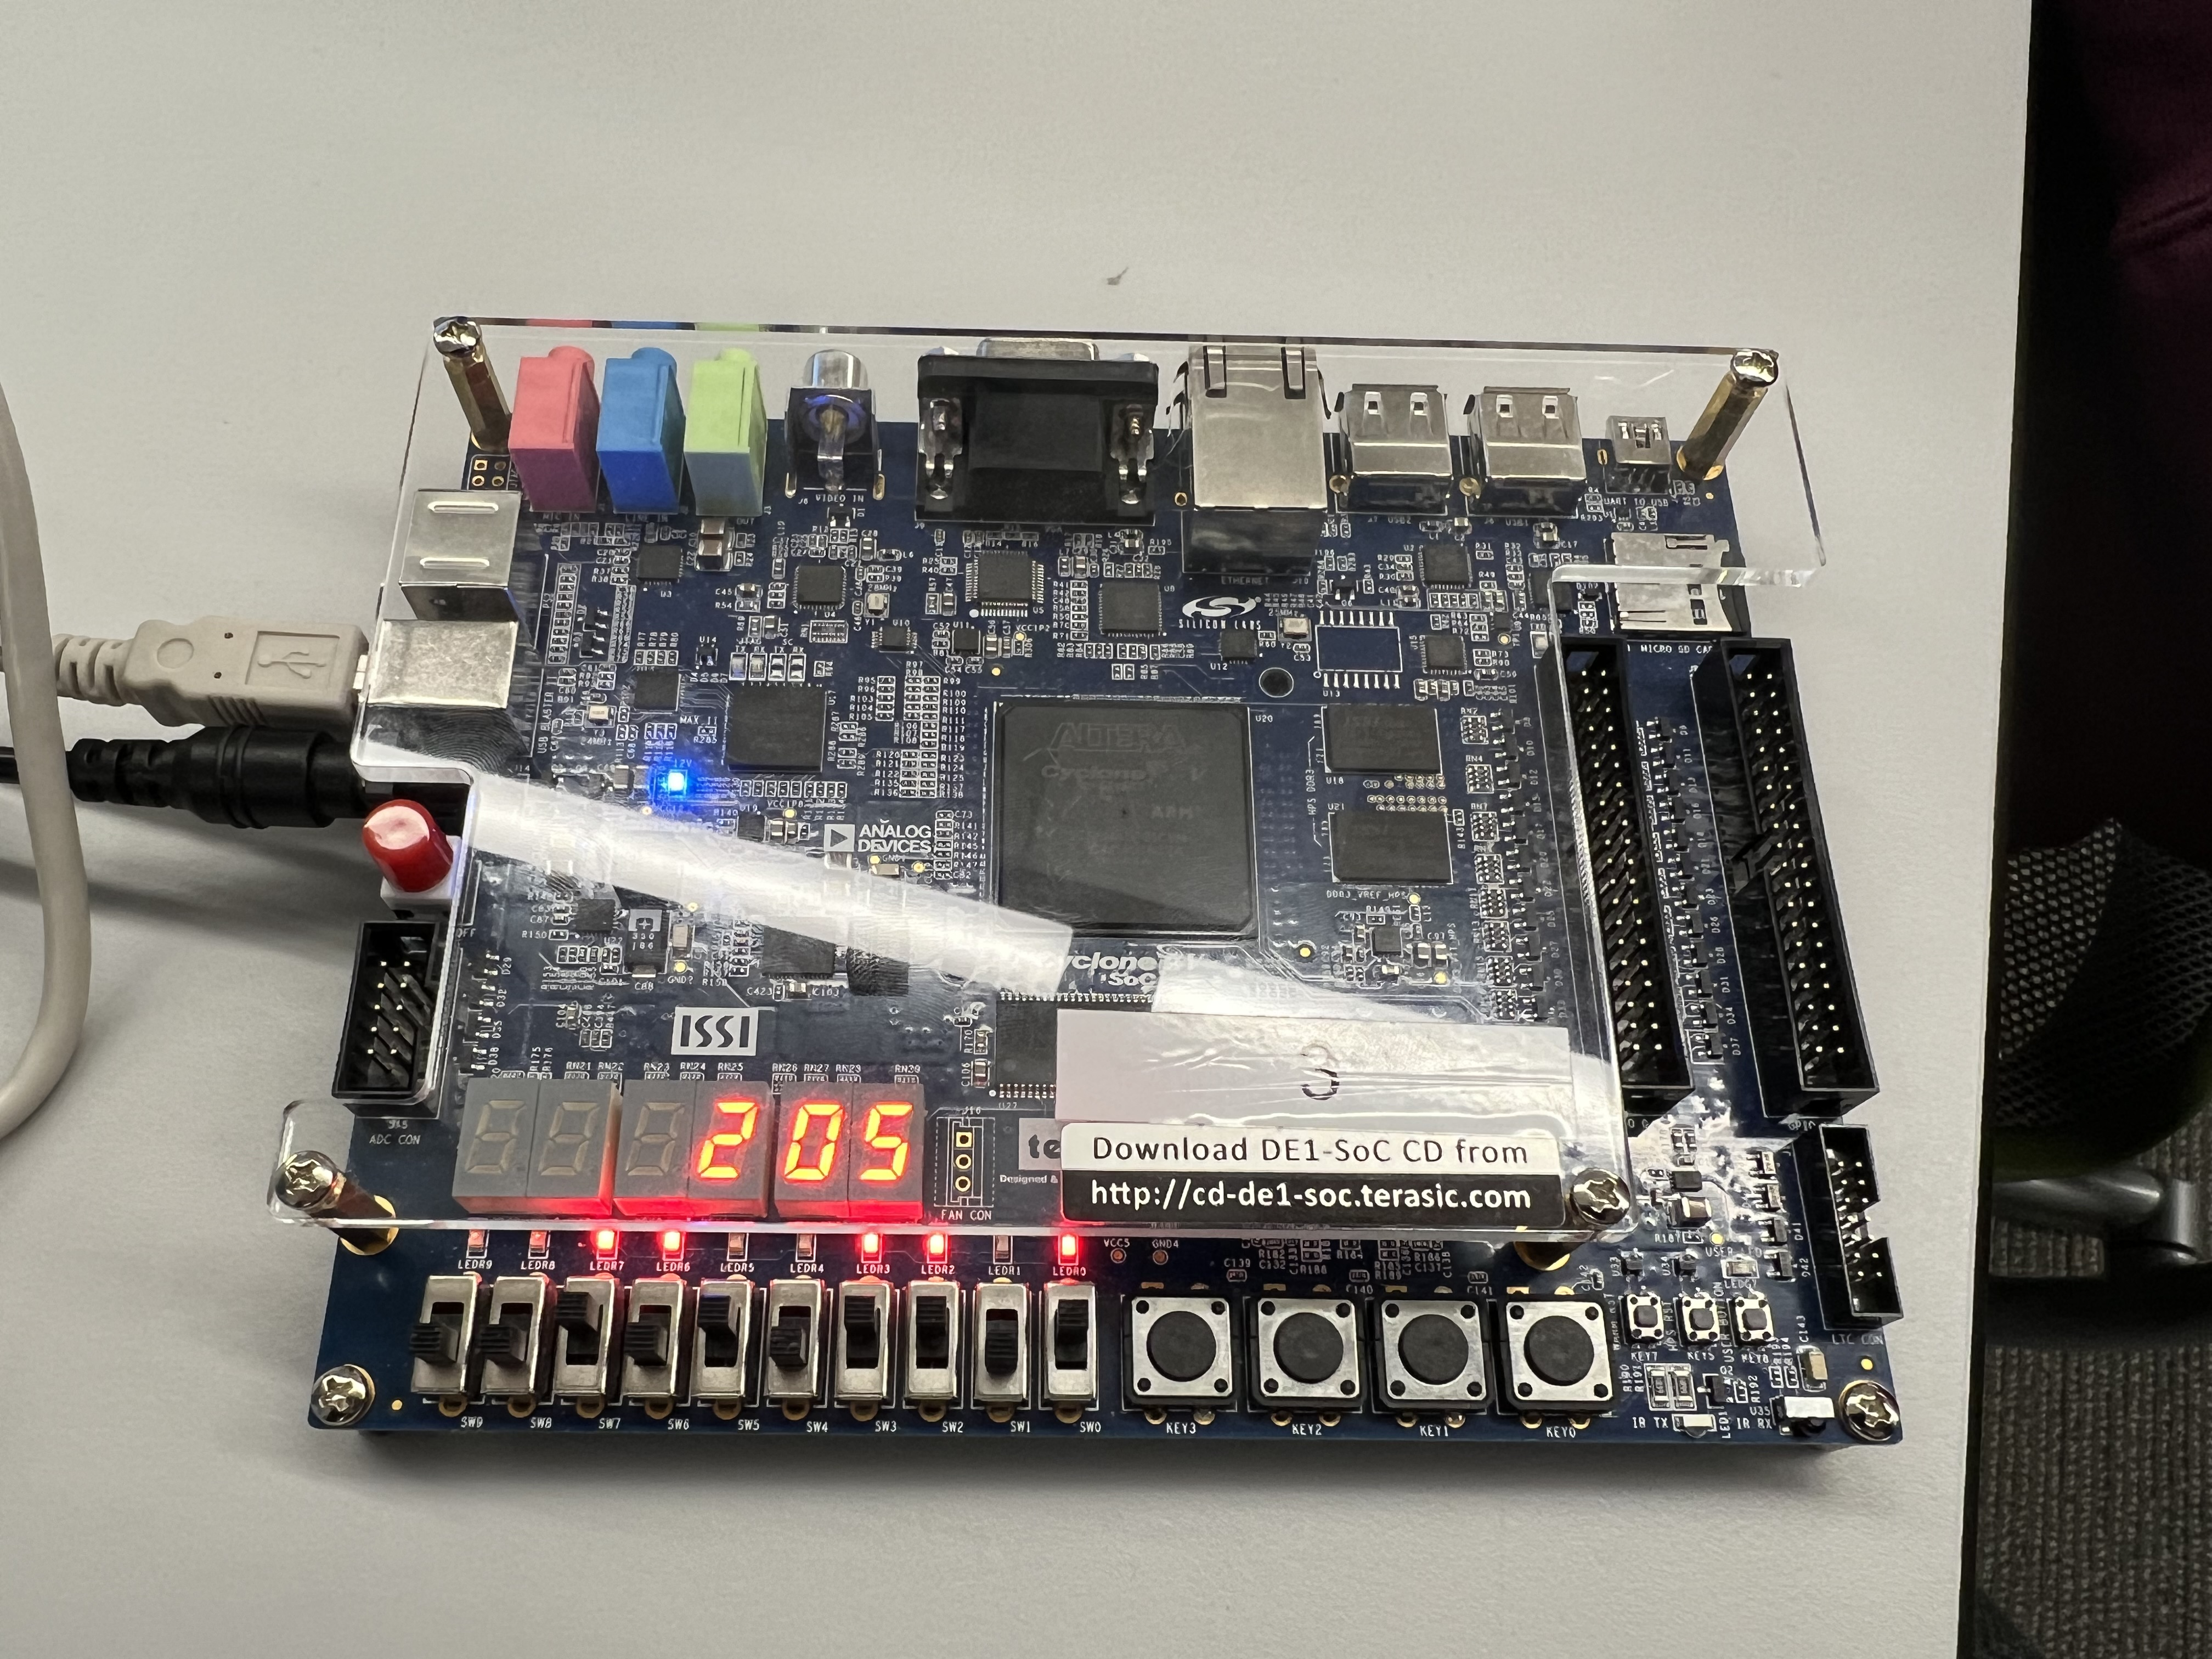
\includegraphics[width=.9\textwidth]{Figures/Part\ 2/IMG_1108.jpg}
  \caption{Addition — Constant $32$ and Binary Input of $10101101_2$ ($173$)}
  \label{fig:9}
\end{figure}

\begin{figure}[H]
  \centering
  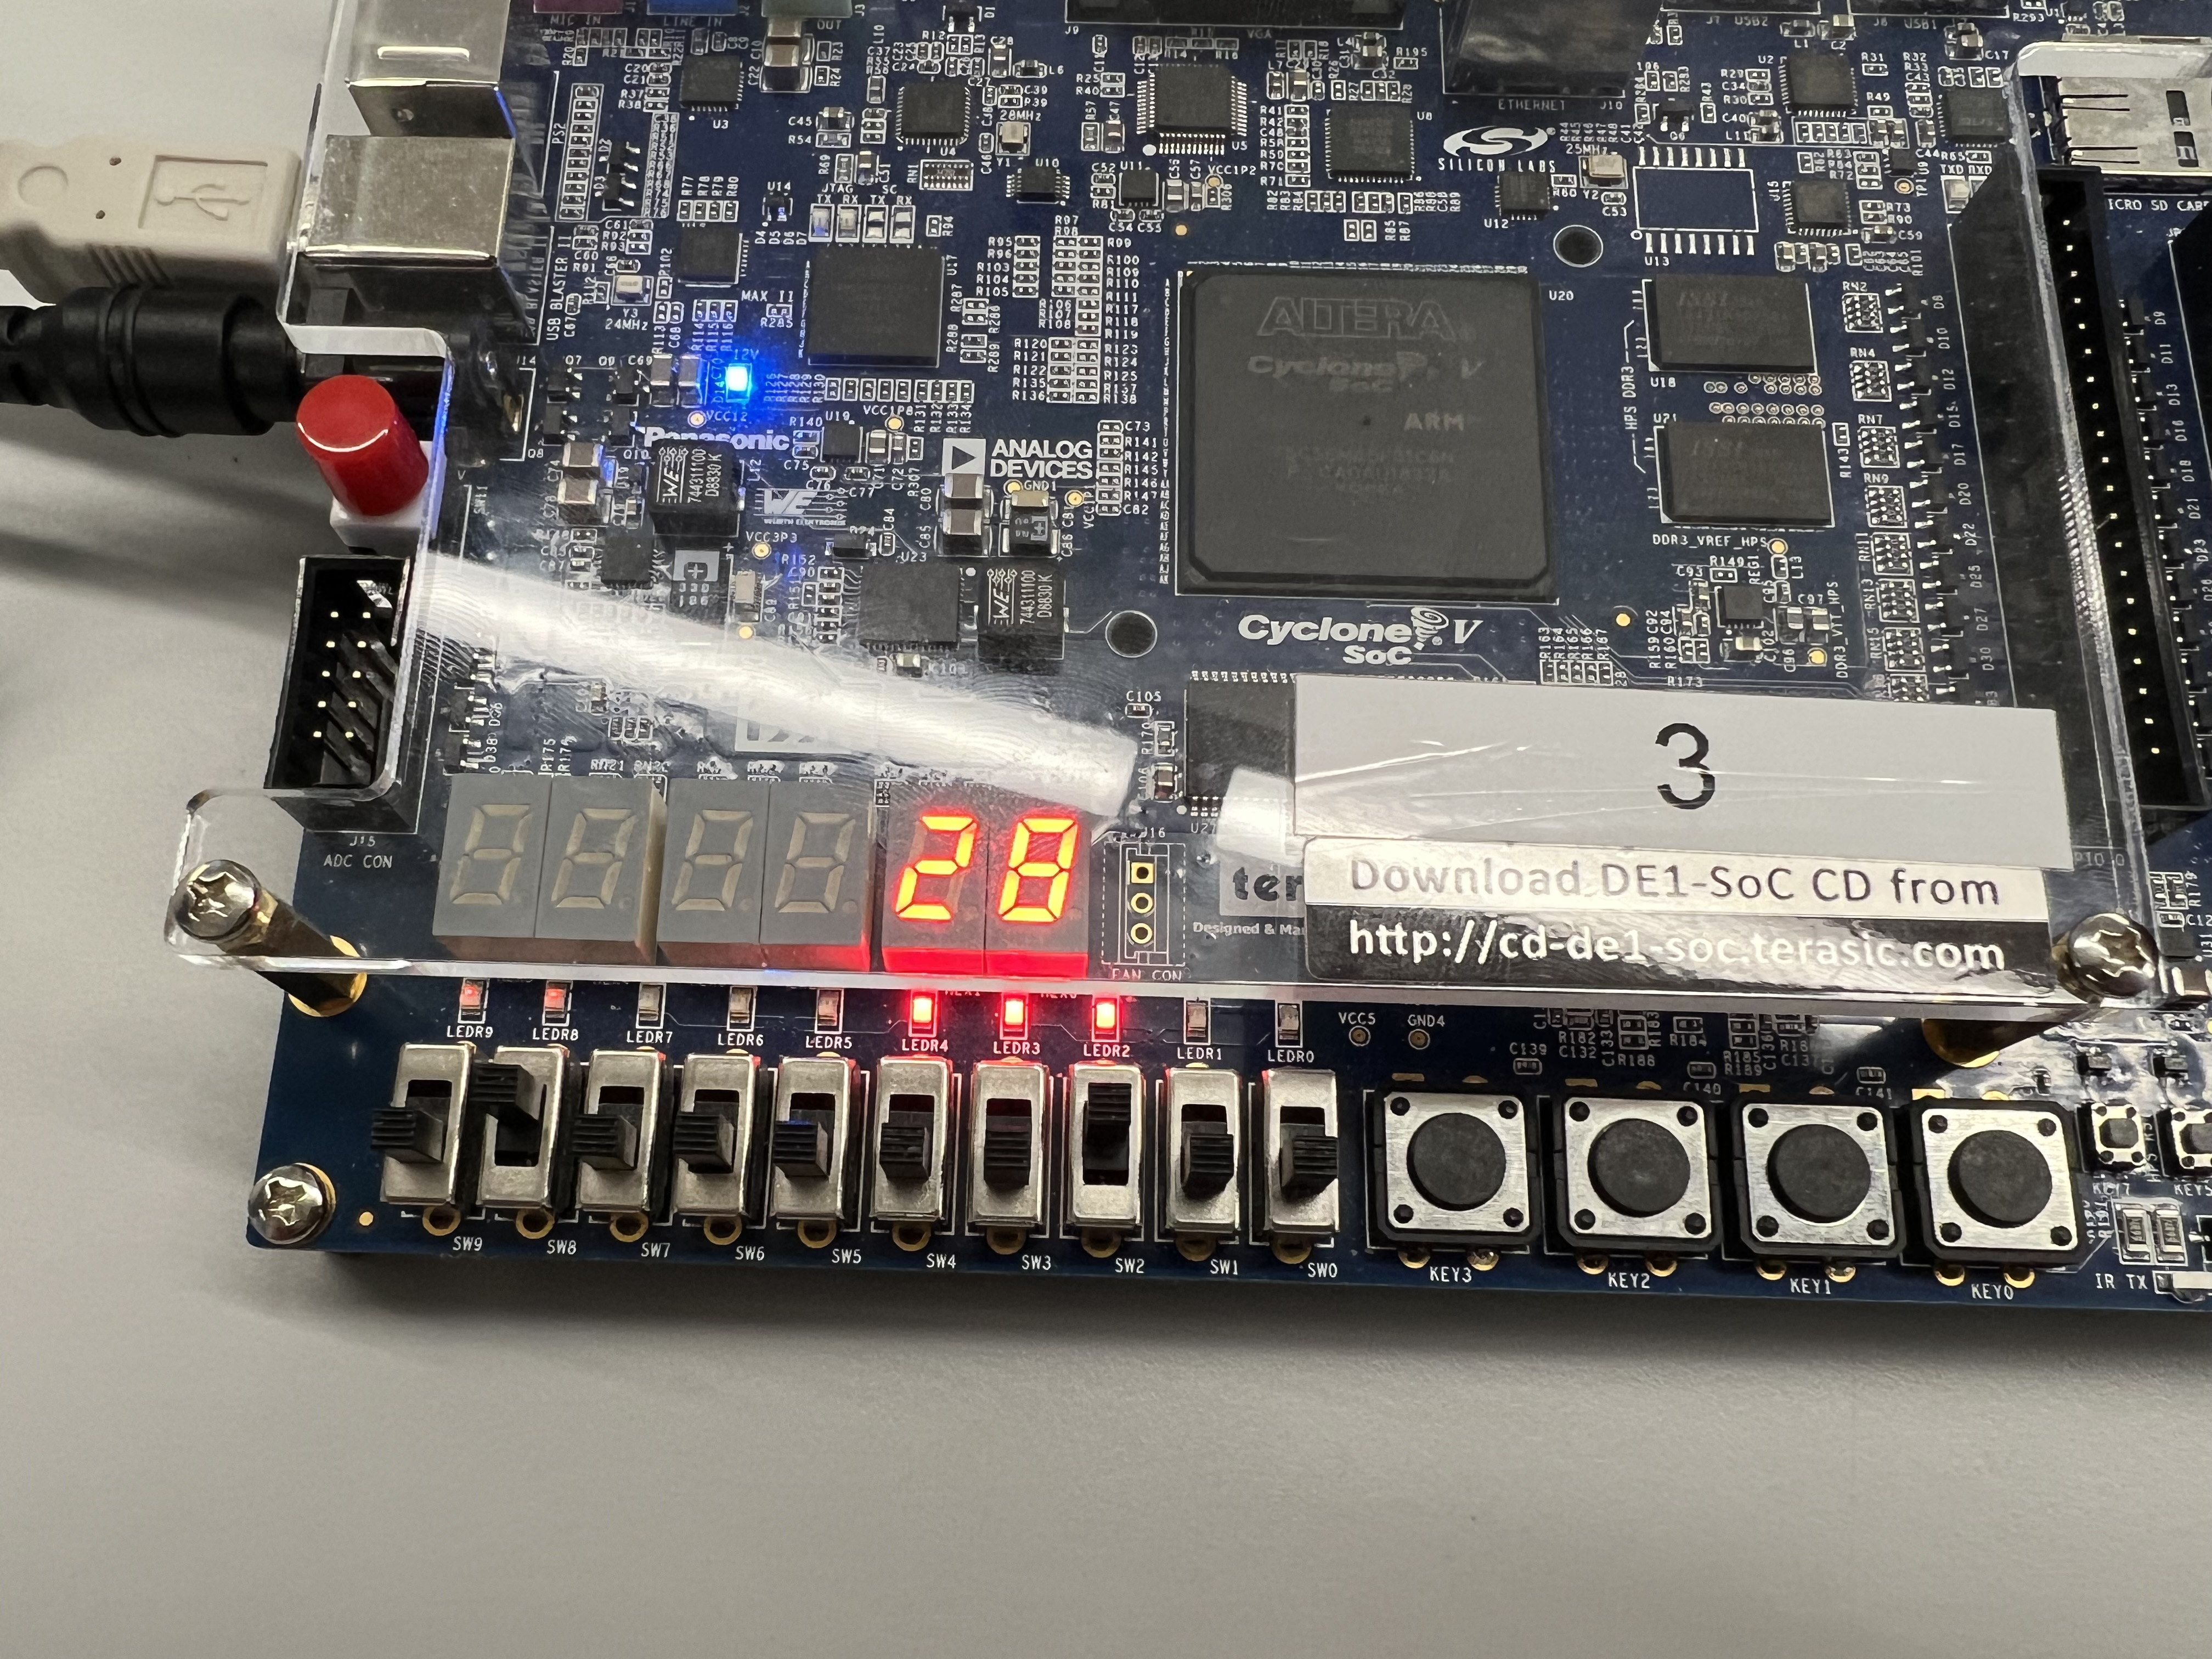
\includegraphics[width=.9\textwidth]{Figures/Part\ 2/IMG_1112.jpg}
  \caption{Subtraction — Constant $32$ minus Binary Input of $00000100_2$ ($4$)}
  \label{fig:10}
\end{figure}

\begin{figure}[H]
  \centering
  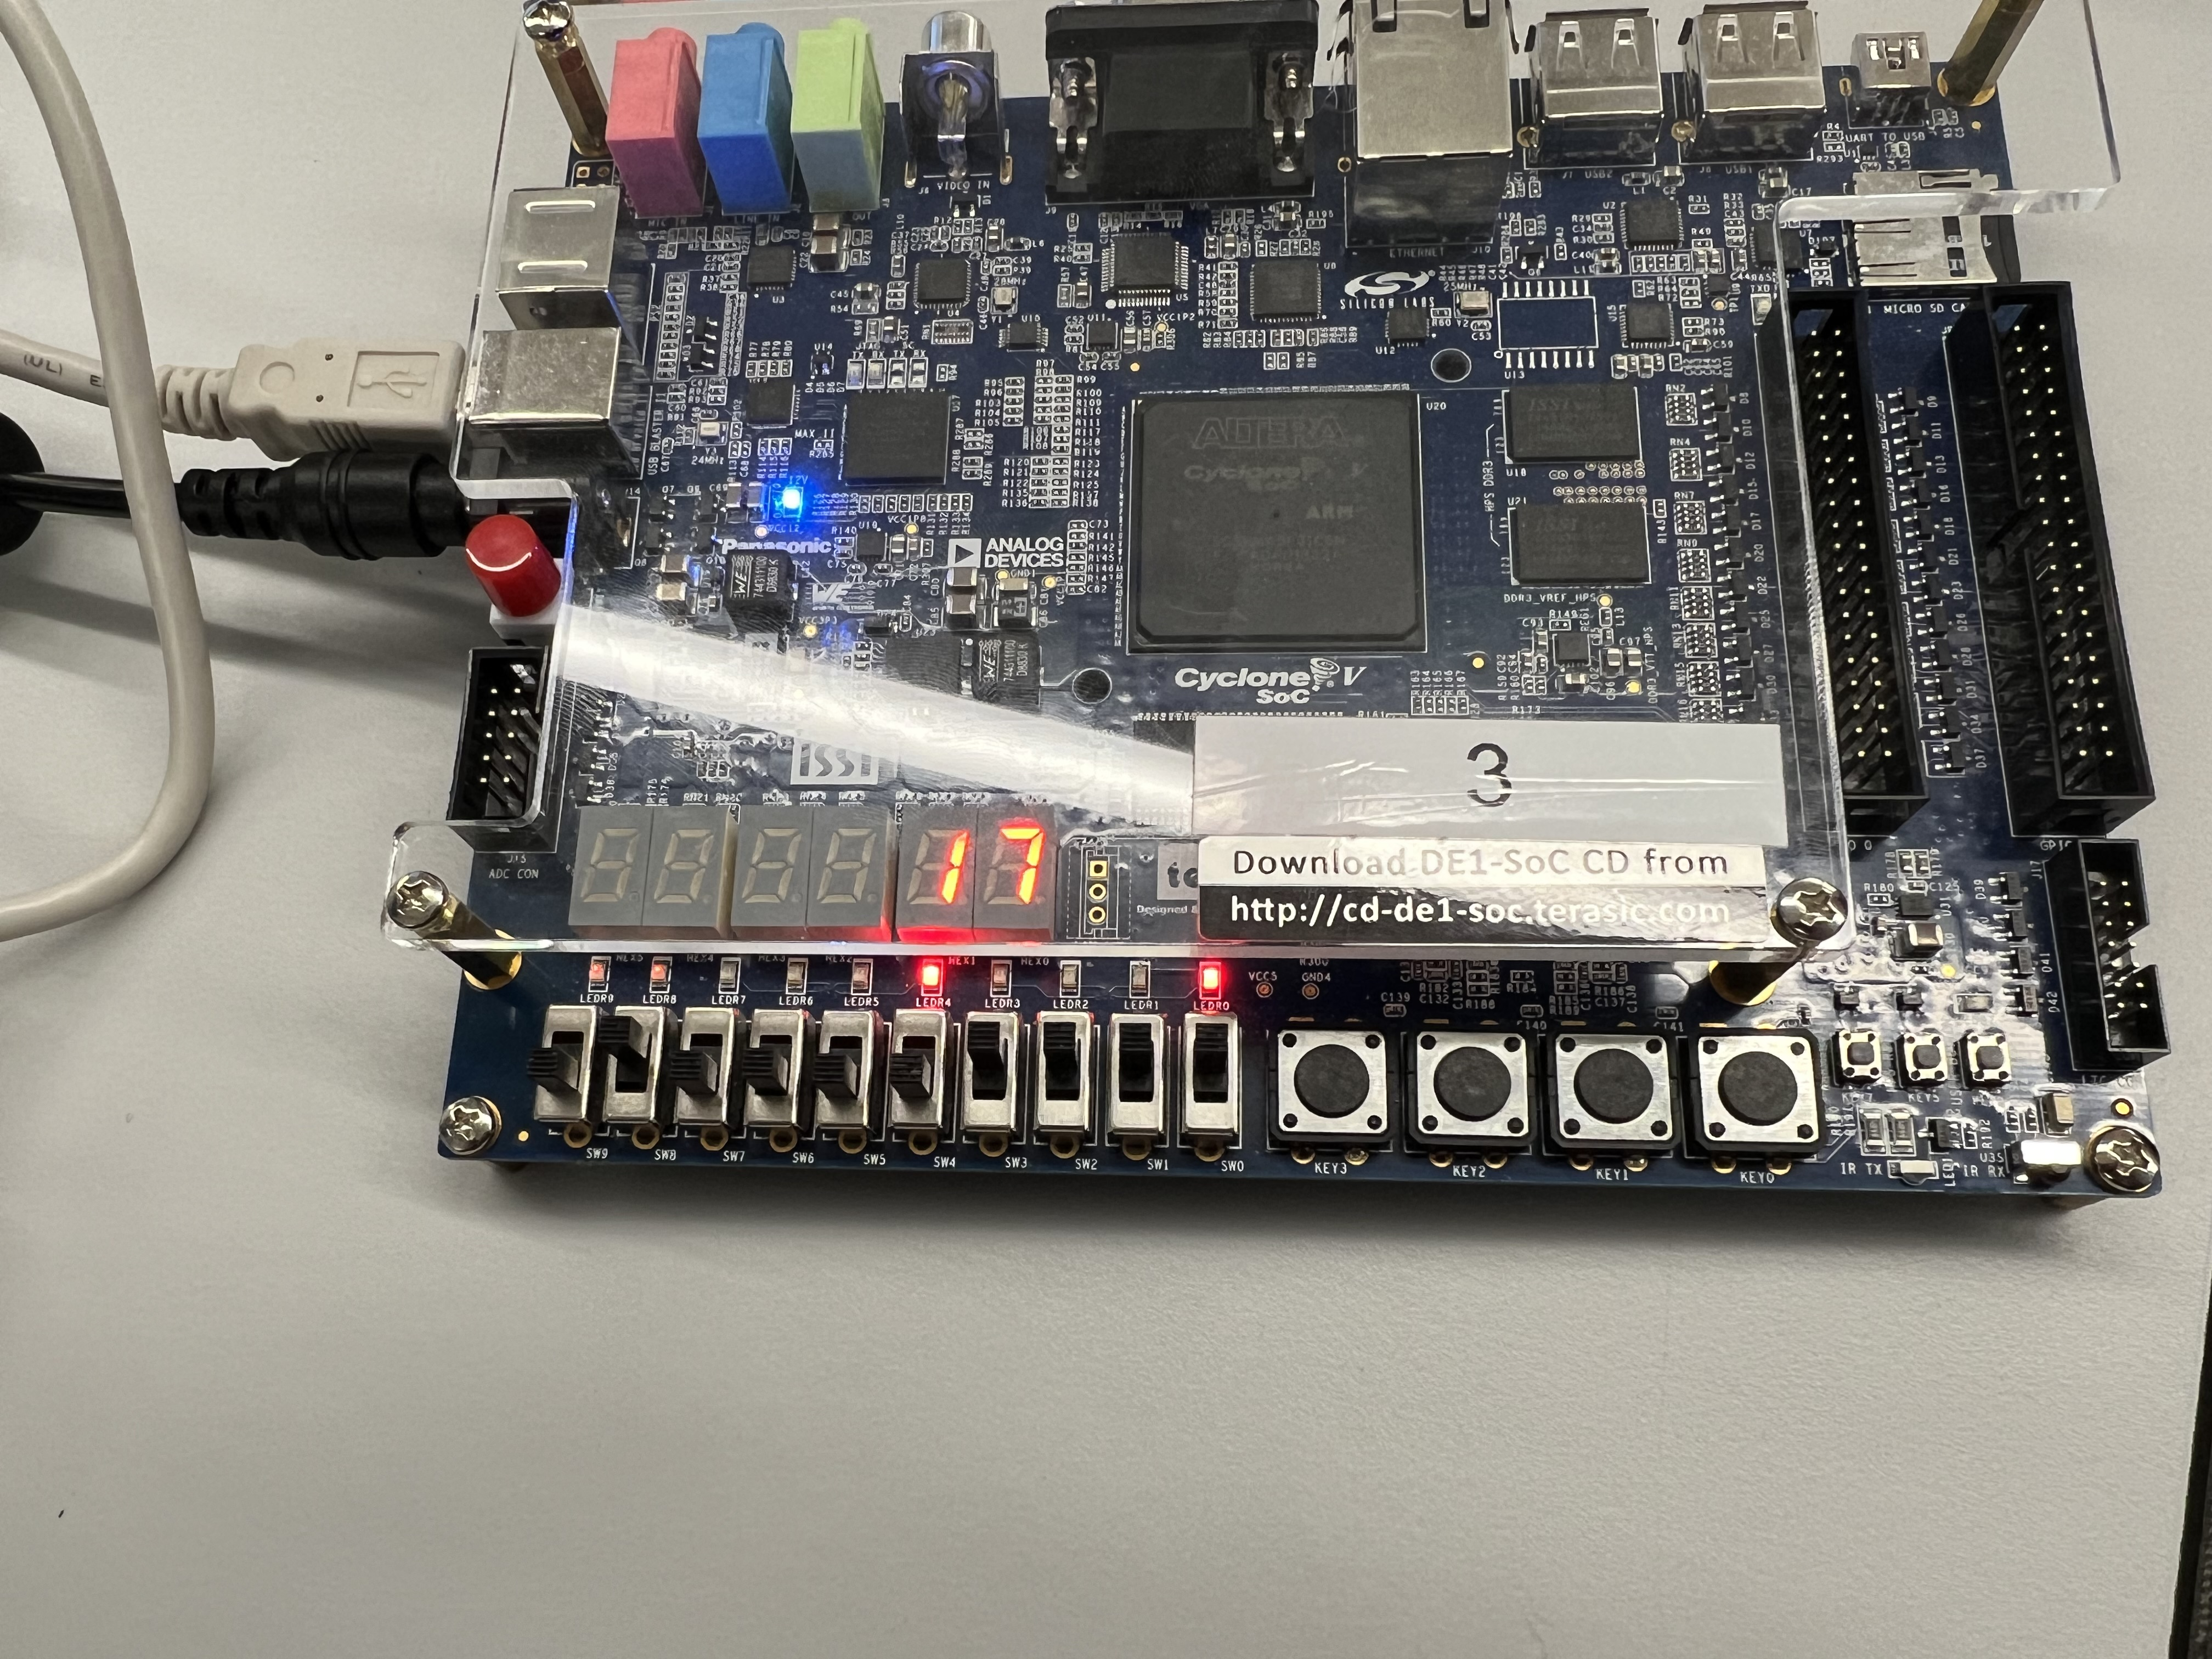
\includegraphics[width=.9\textwidth]{Figures/Part\ 2/IMG_1113.jpg}
  \caption{Subtraction — Constant $32$ minus Binary Input of $00001111_2$ ($15$)}
  \label{fig:11}
\end{figure}

\begin{figure}[H]
  \centering
  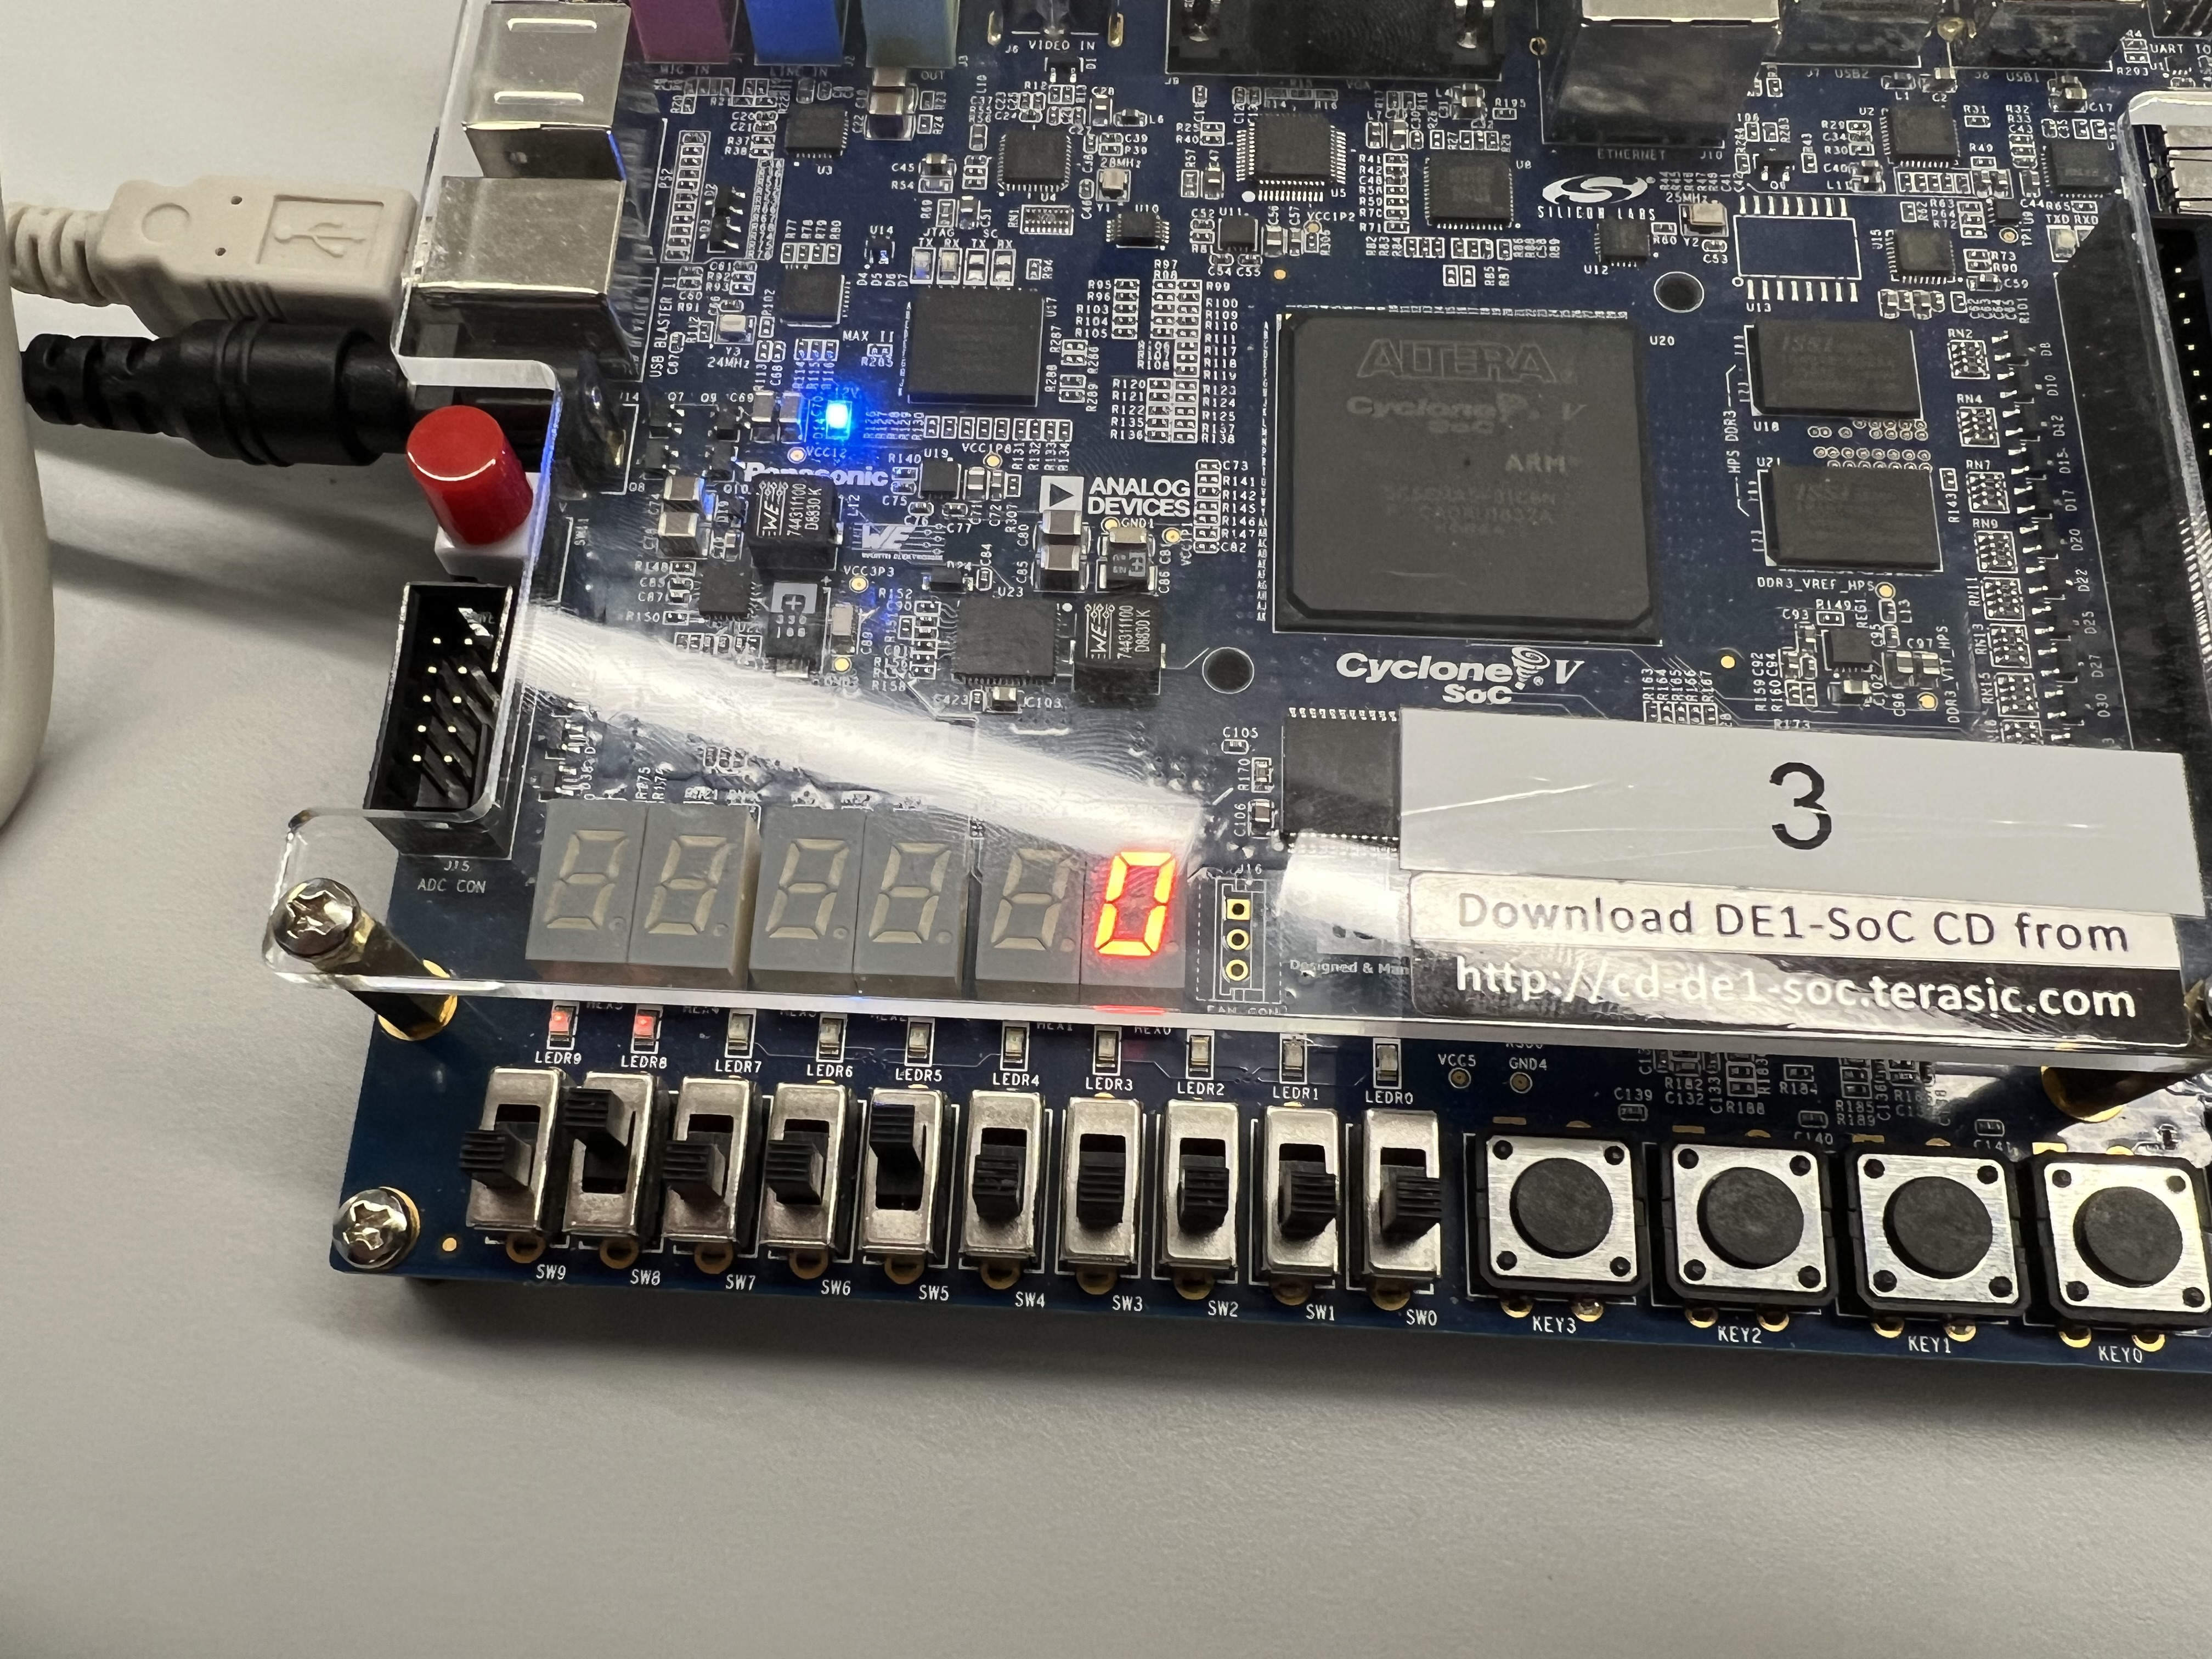
\includegraphics[width=.9\textwidth]{Figures/Part\ 2/IMG_1111.jpg}
  \caption{Subtraction — Constant $32$ minus Binary Input of $00100000_2$ ($32$)}
  \label{fig:12}
\end{figure}

\begin{figure}[H]
  \centering
  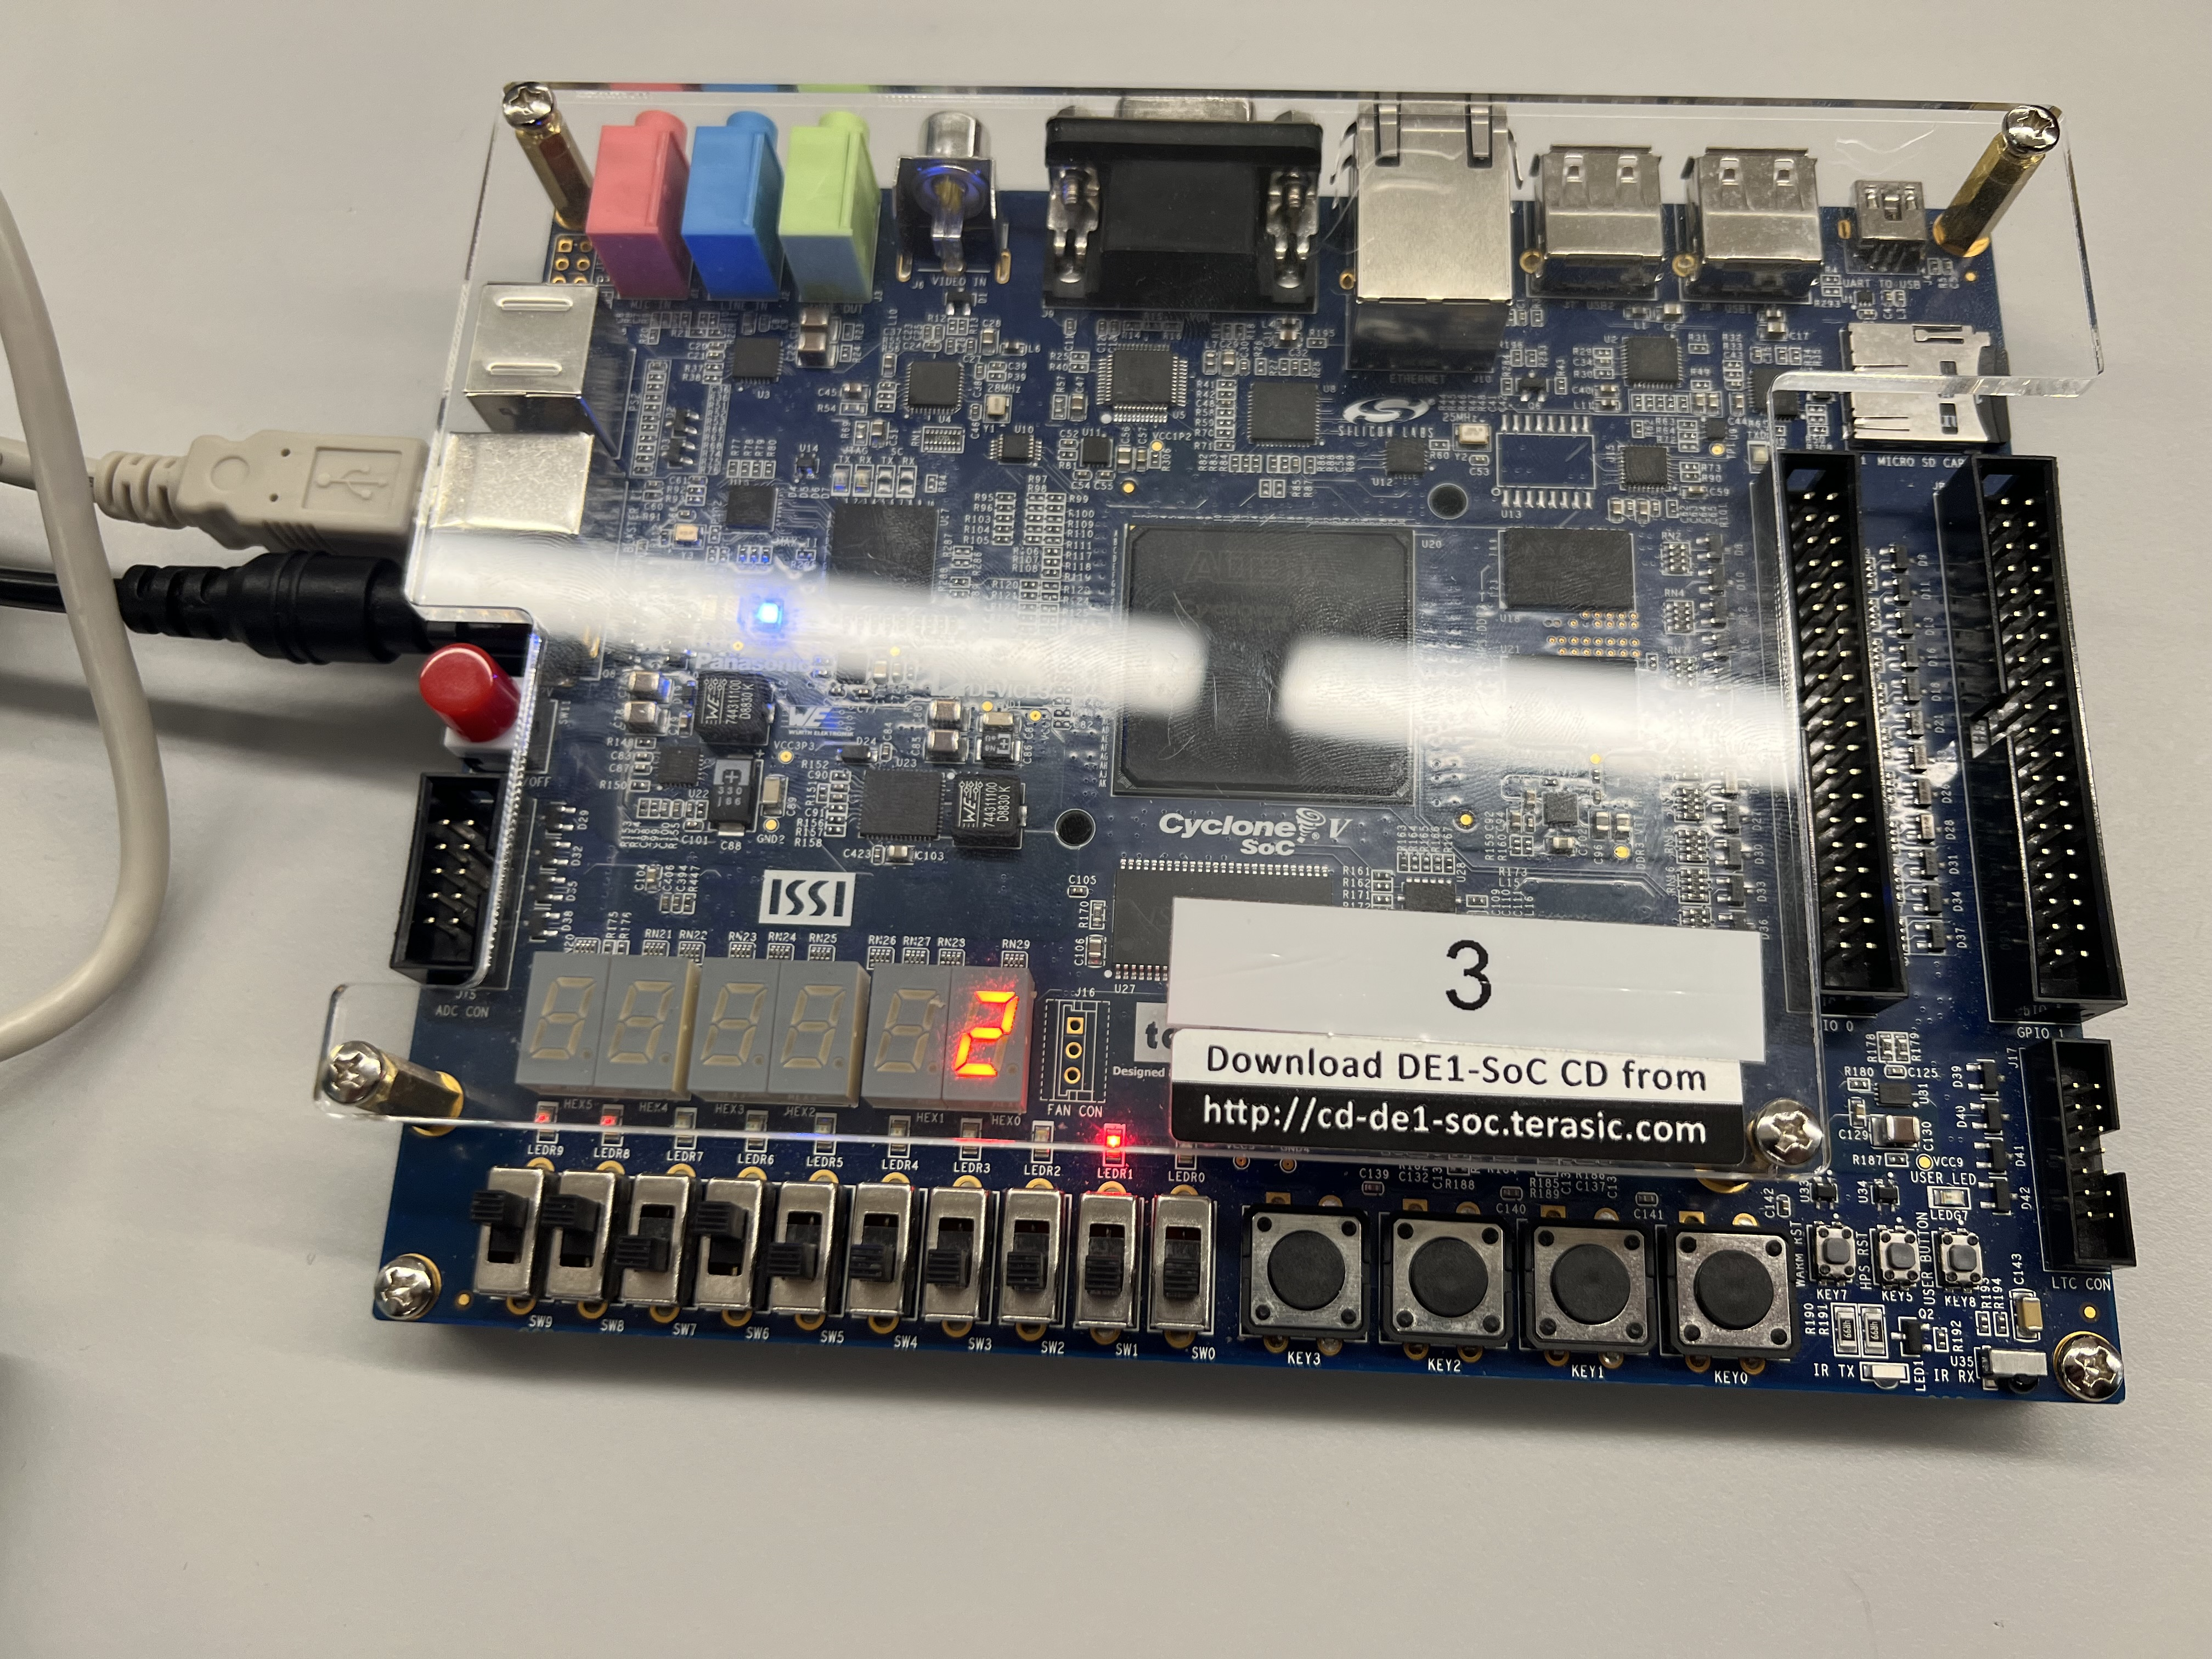
\includegraphics[width=.9\textwidth]{Figures/Part\ 2/IMG_1115.jpg}
  \caption{Division — Binary Input of $01000000_2$ ($64$) Divided by the Constant $32$}
  \label{fig:13}
\end{figure}

\begin{figure}[H]
  \centering
  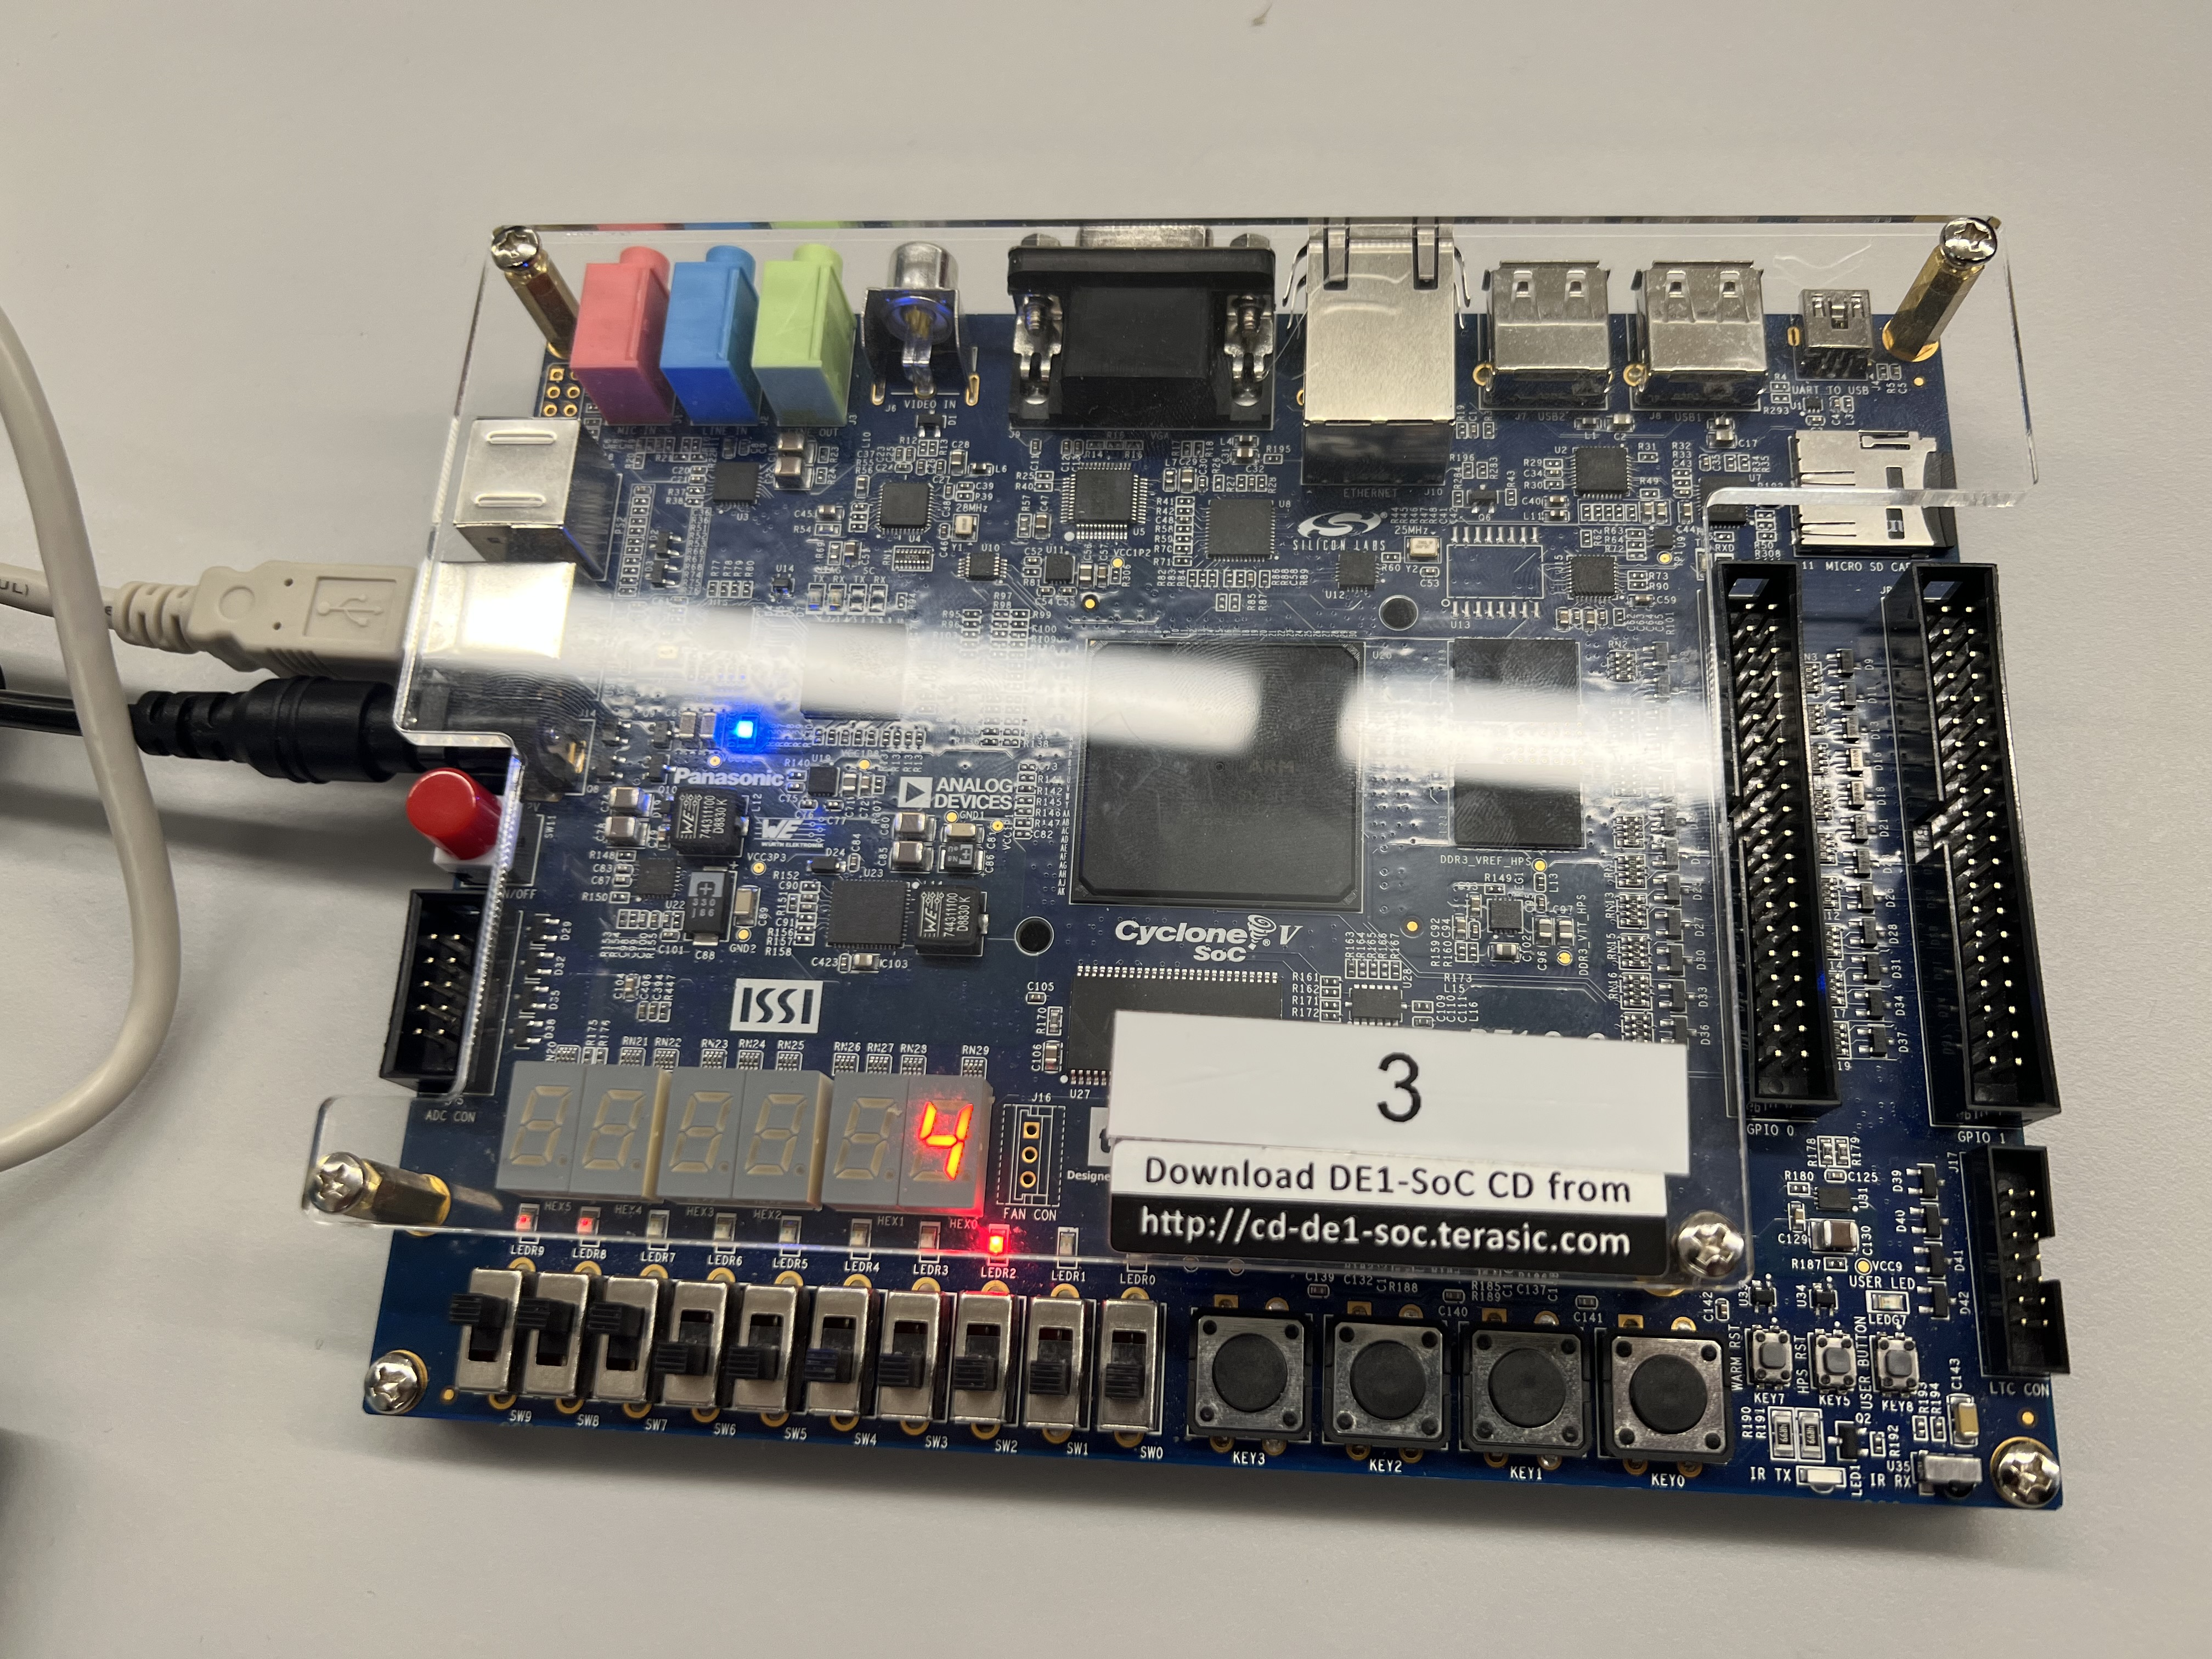
\includegraphics[width=.9\textwidth]{Figures/Part\ 2/IMG_1114.jpg}
  \caption{Division — Binary Input of $10000000_2$ ($128$) Divided by the Constant $32$}
  \label{fig:14}
\end{figure}

\begin{figure}[H]
  \centering
  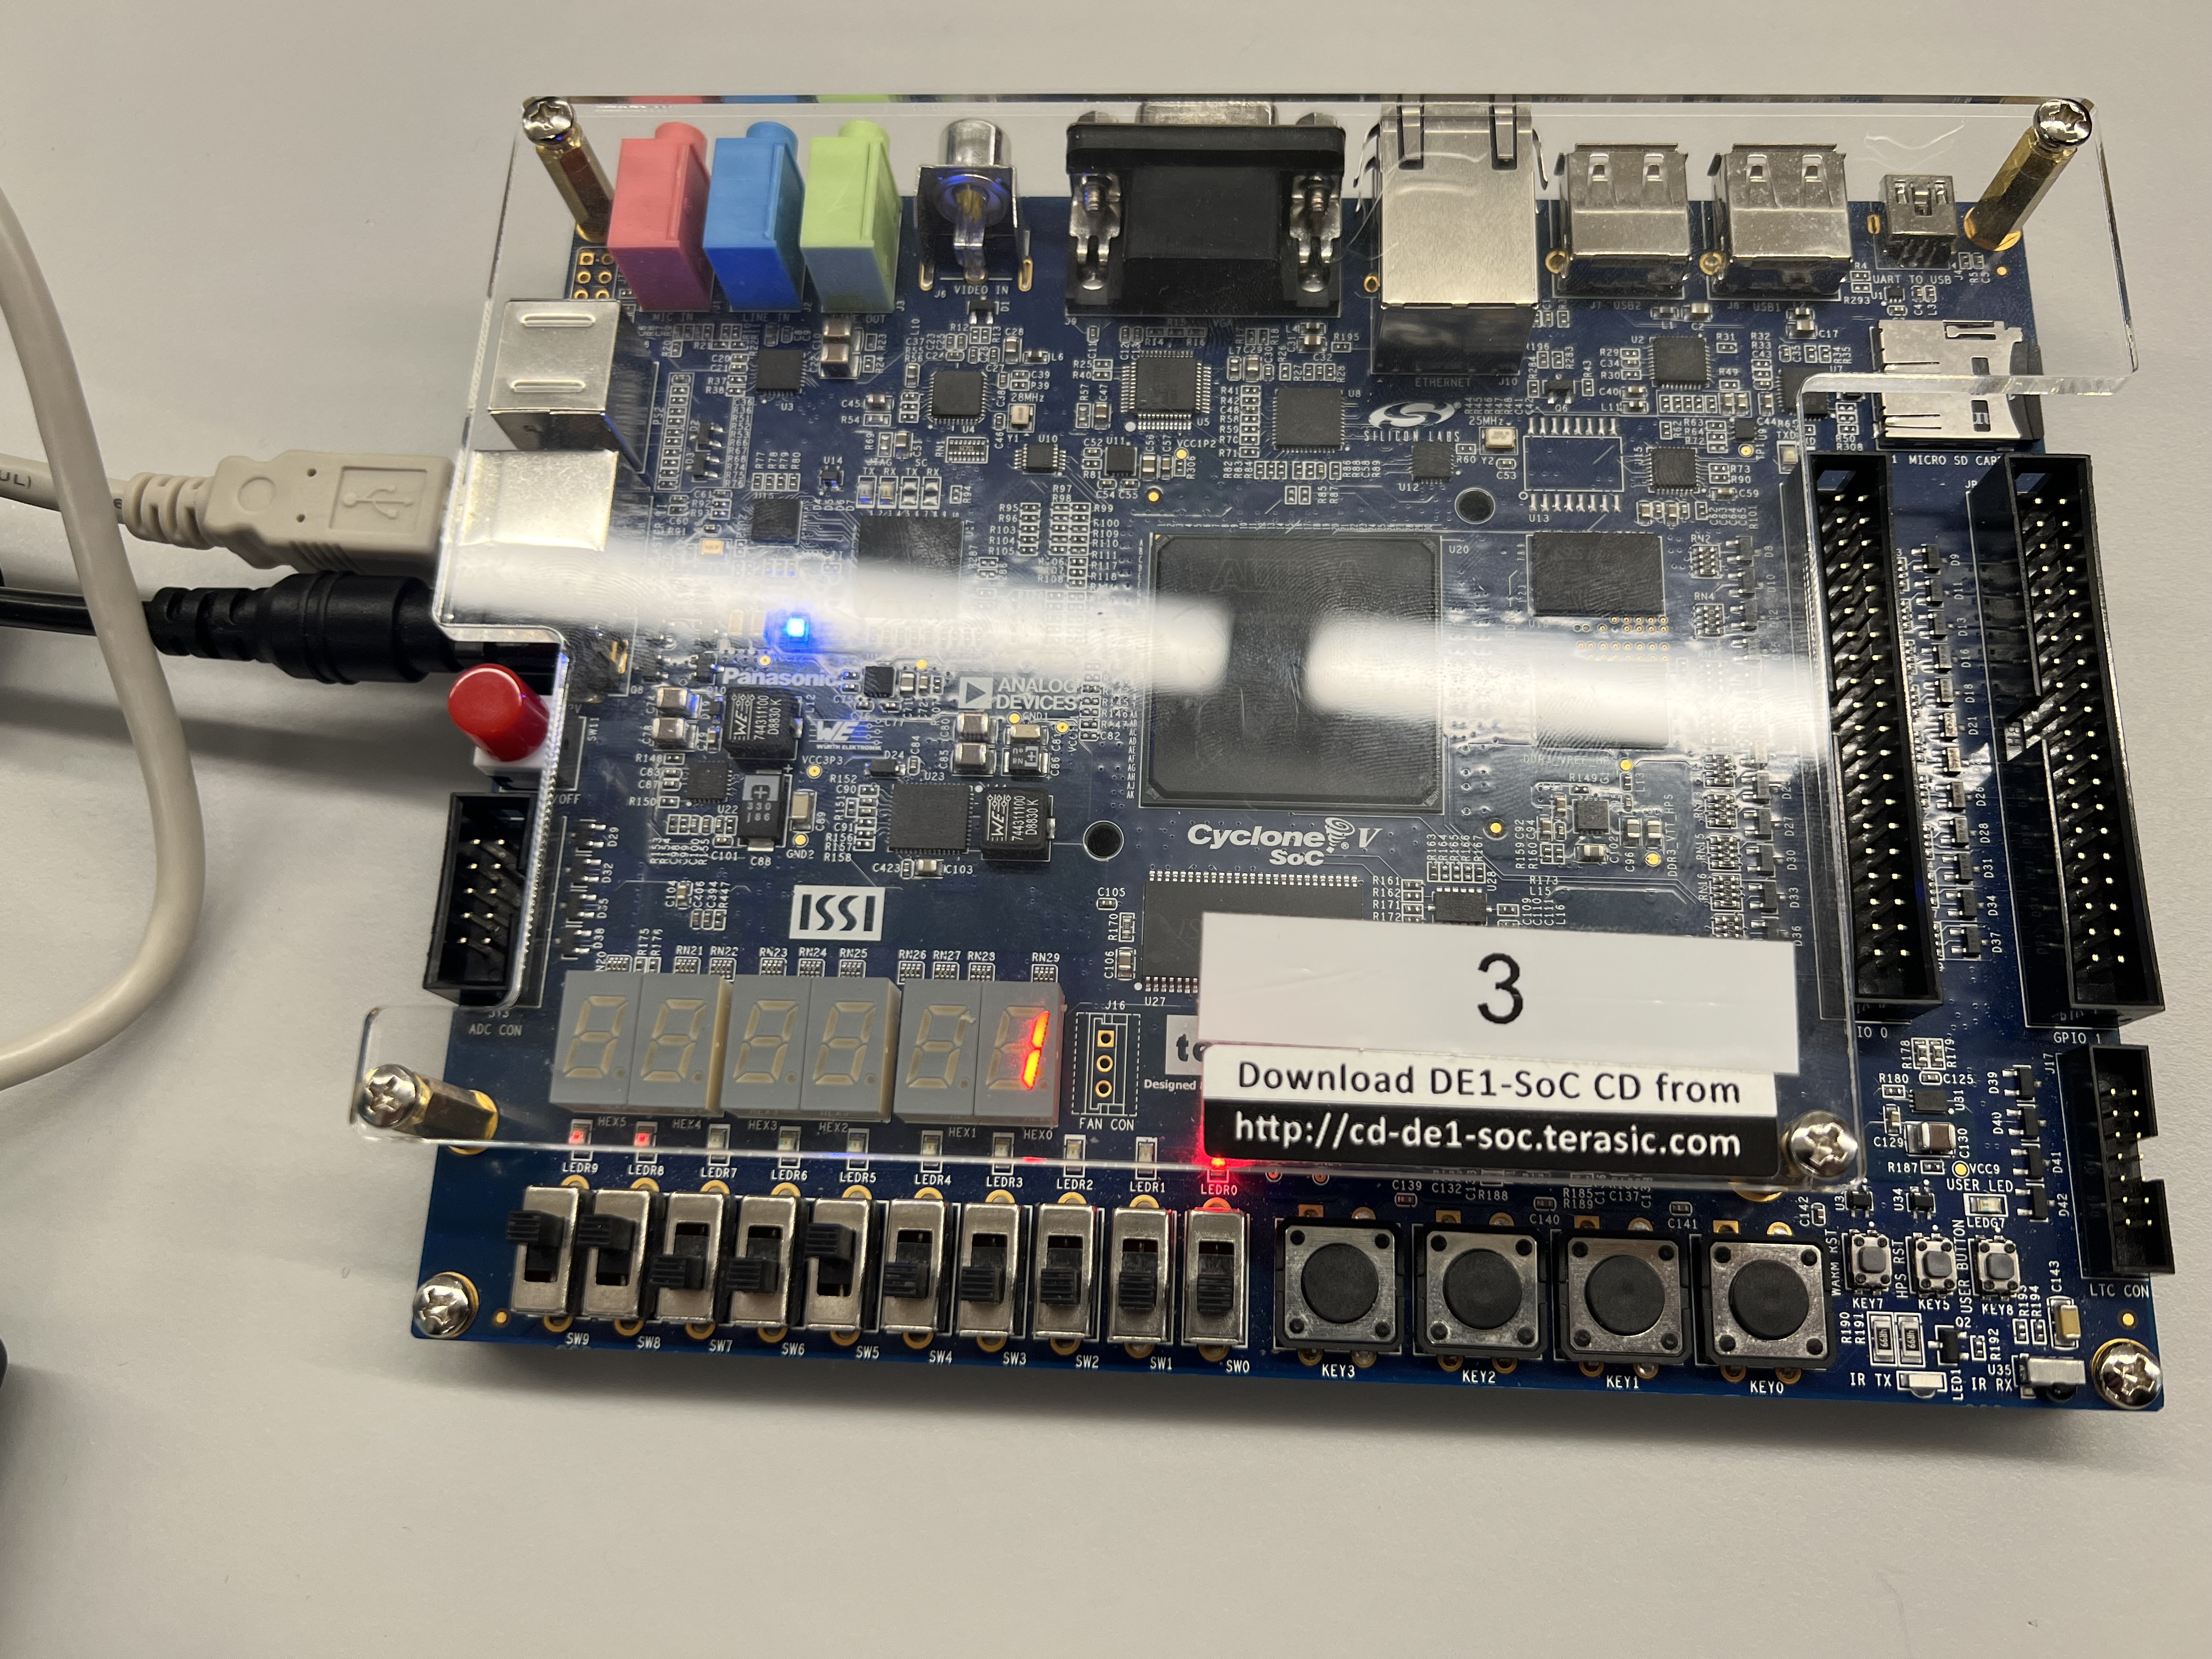
\includegraphics[width=.9\textwidth]{Figures/Part\ 2/IMG_1116.jpg}
  \caption{Division — Binary Input of$ 00100000_2$ ($32$) Divided by the Constant $32$}
  \label{fig:15}
\end{figure}

\begin{figure}[H]
  \centering
  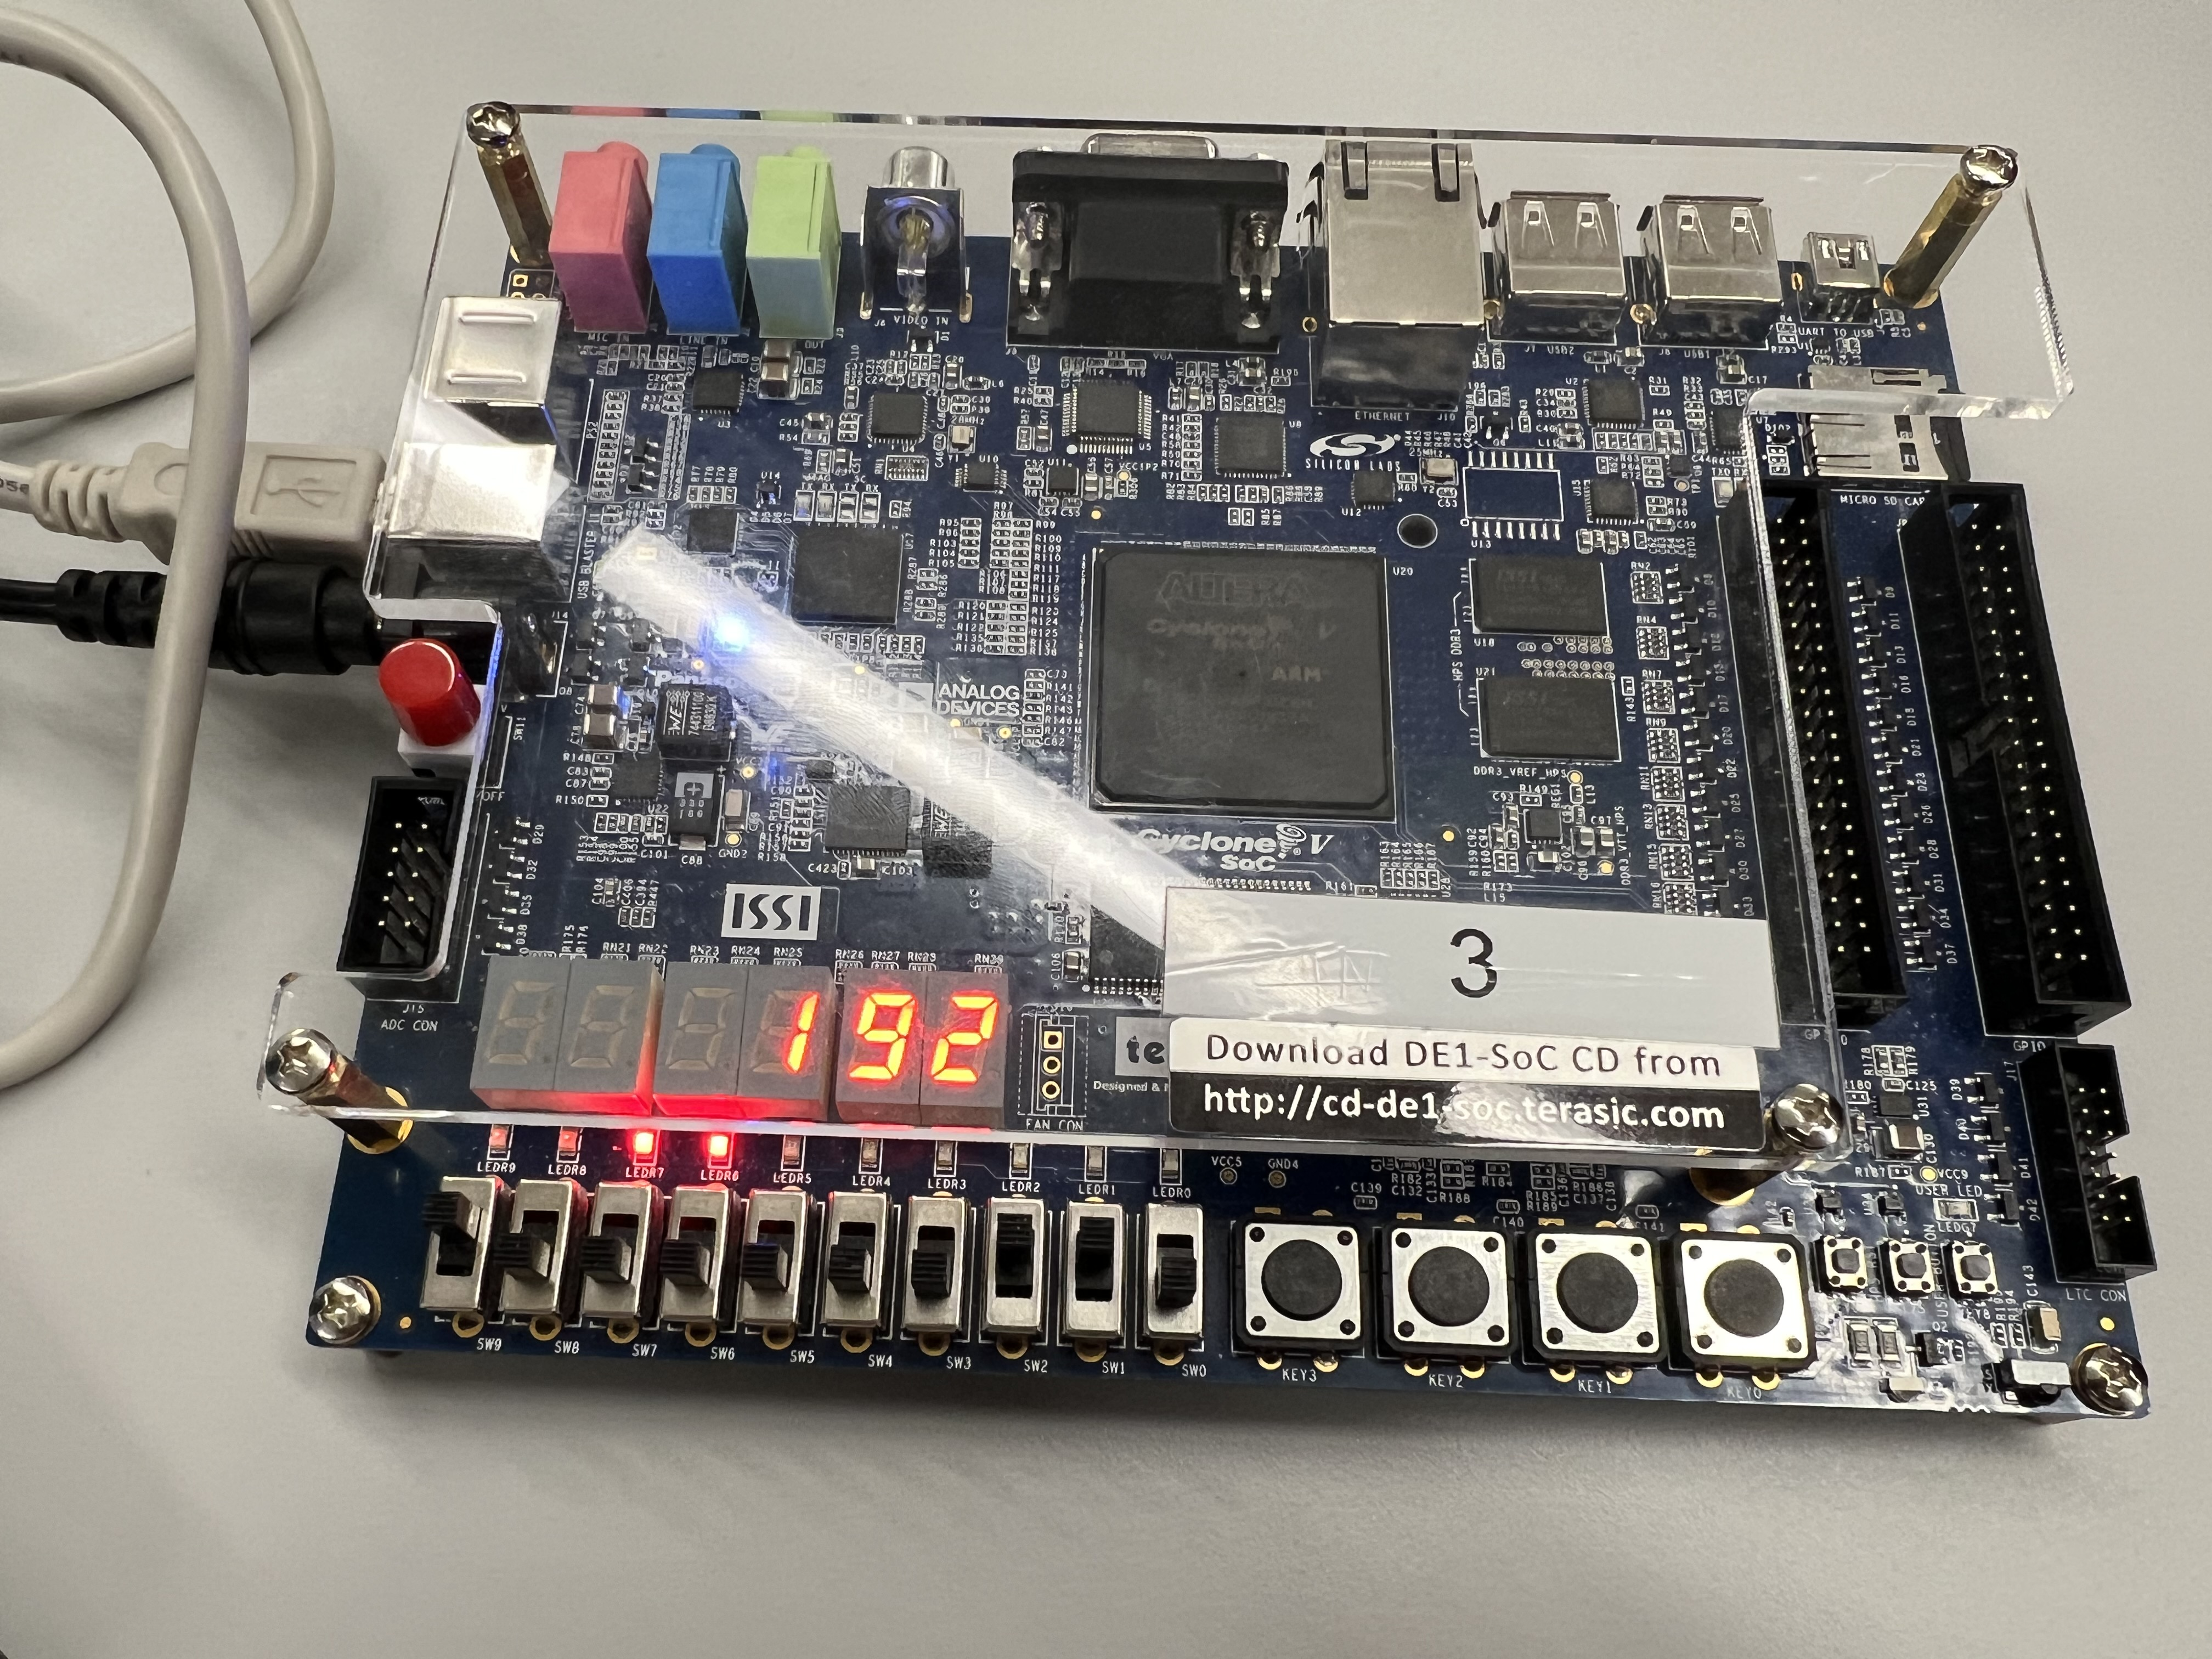
\includegraphics[width=.9\textwidth]{Figures/Part\ 2/IMG_1119.jpg}
  \caption{Multiplication — Binary Input of $00000110_2$ ($6$) and the Constant $32$}
  \label{fig:16}
\end{figure}

\begin{figure}[H]
  \centering
  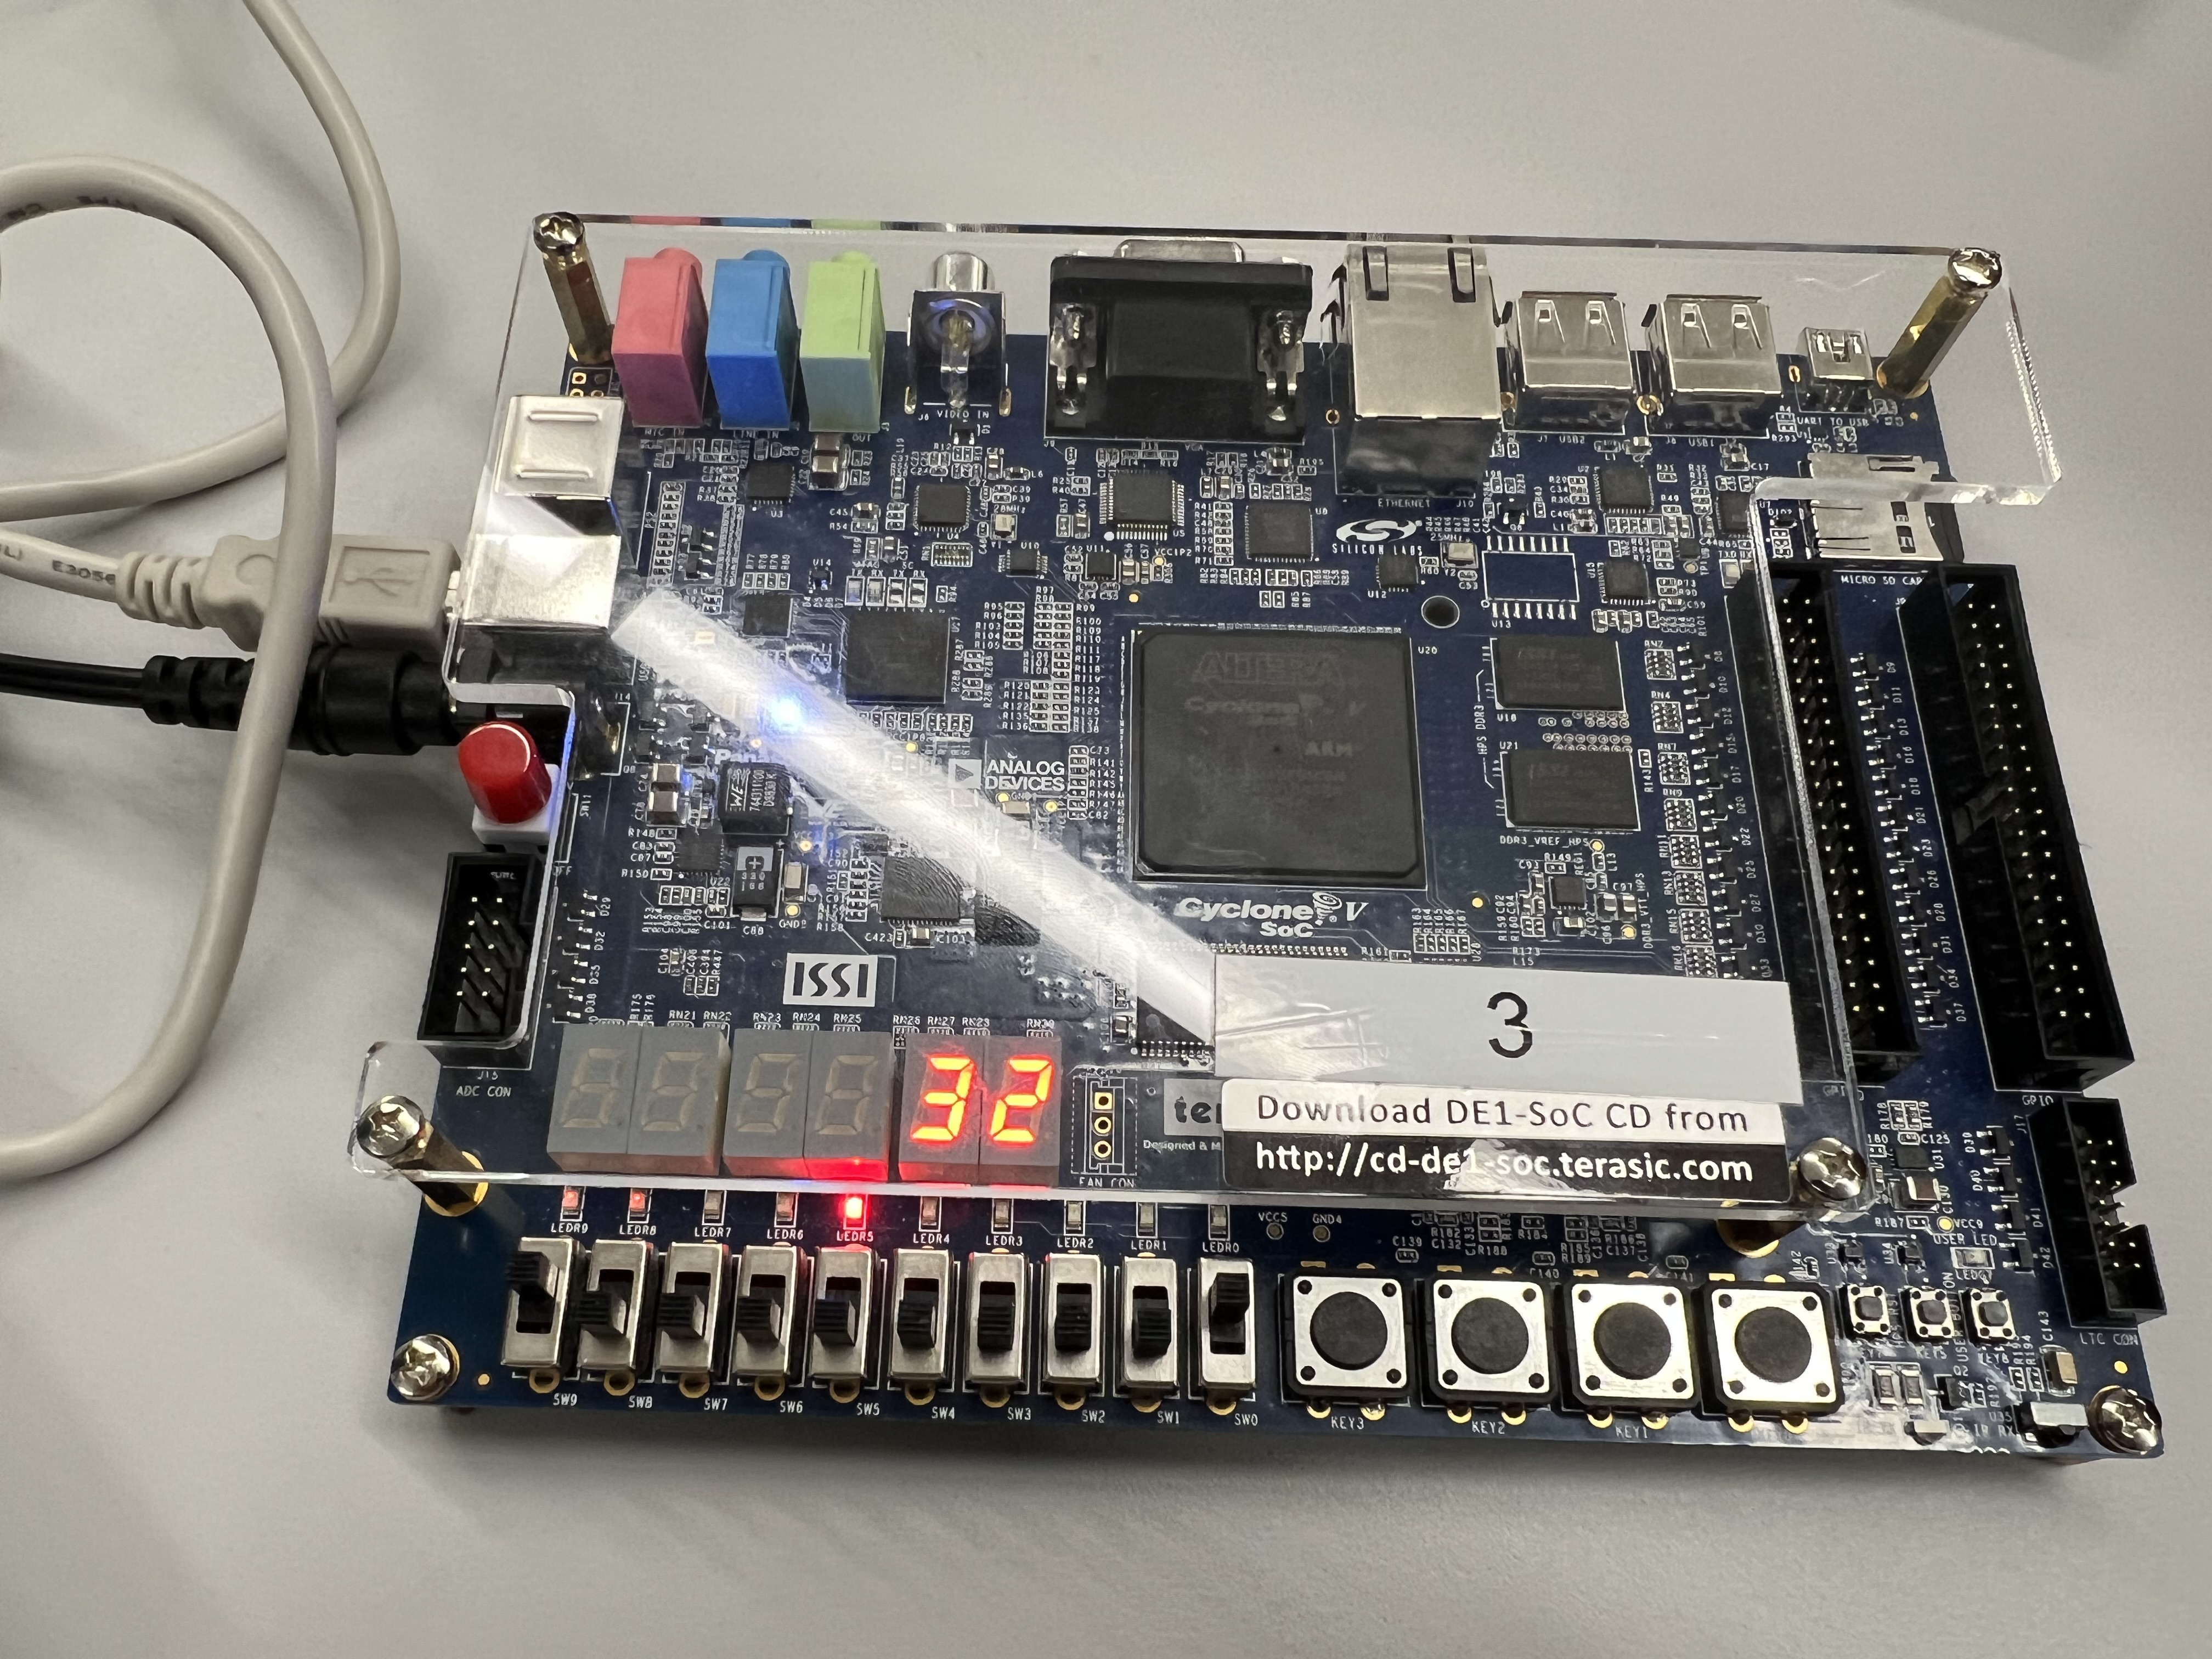
\includegraphics[width=.9\textwidth]{Figures/Part\ 2/IMG_1118.jpg}
  \caption{Multiplication —  Binary Input of $00000001_2$ ($1$) and the Constant $32$}
  \label{fig:17}
\end{figure}

\begin{figure}[H]
  \centering
  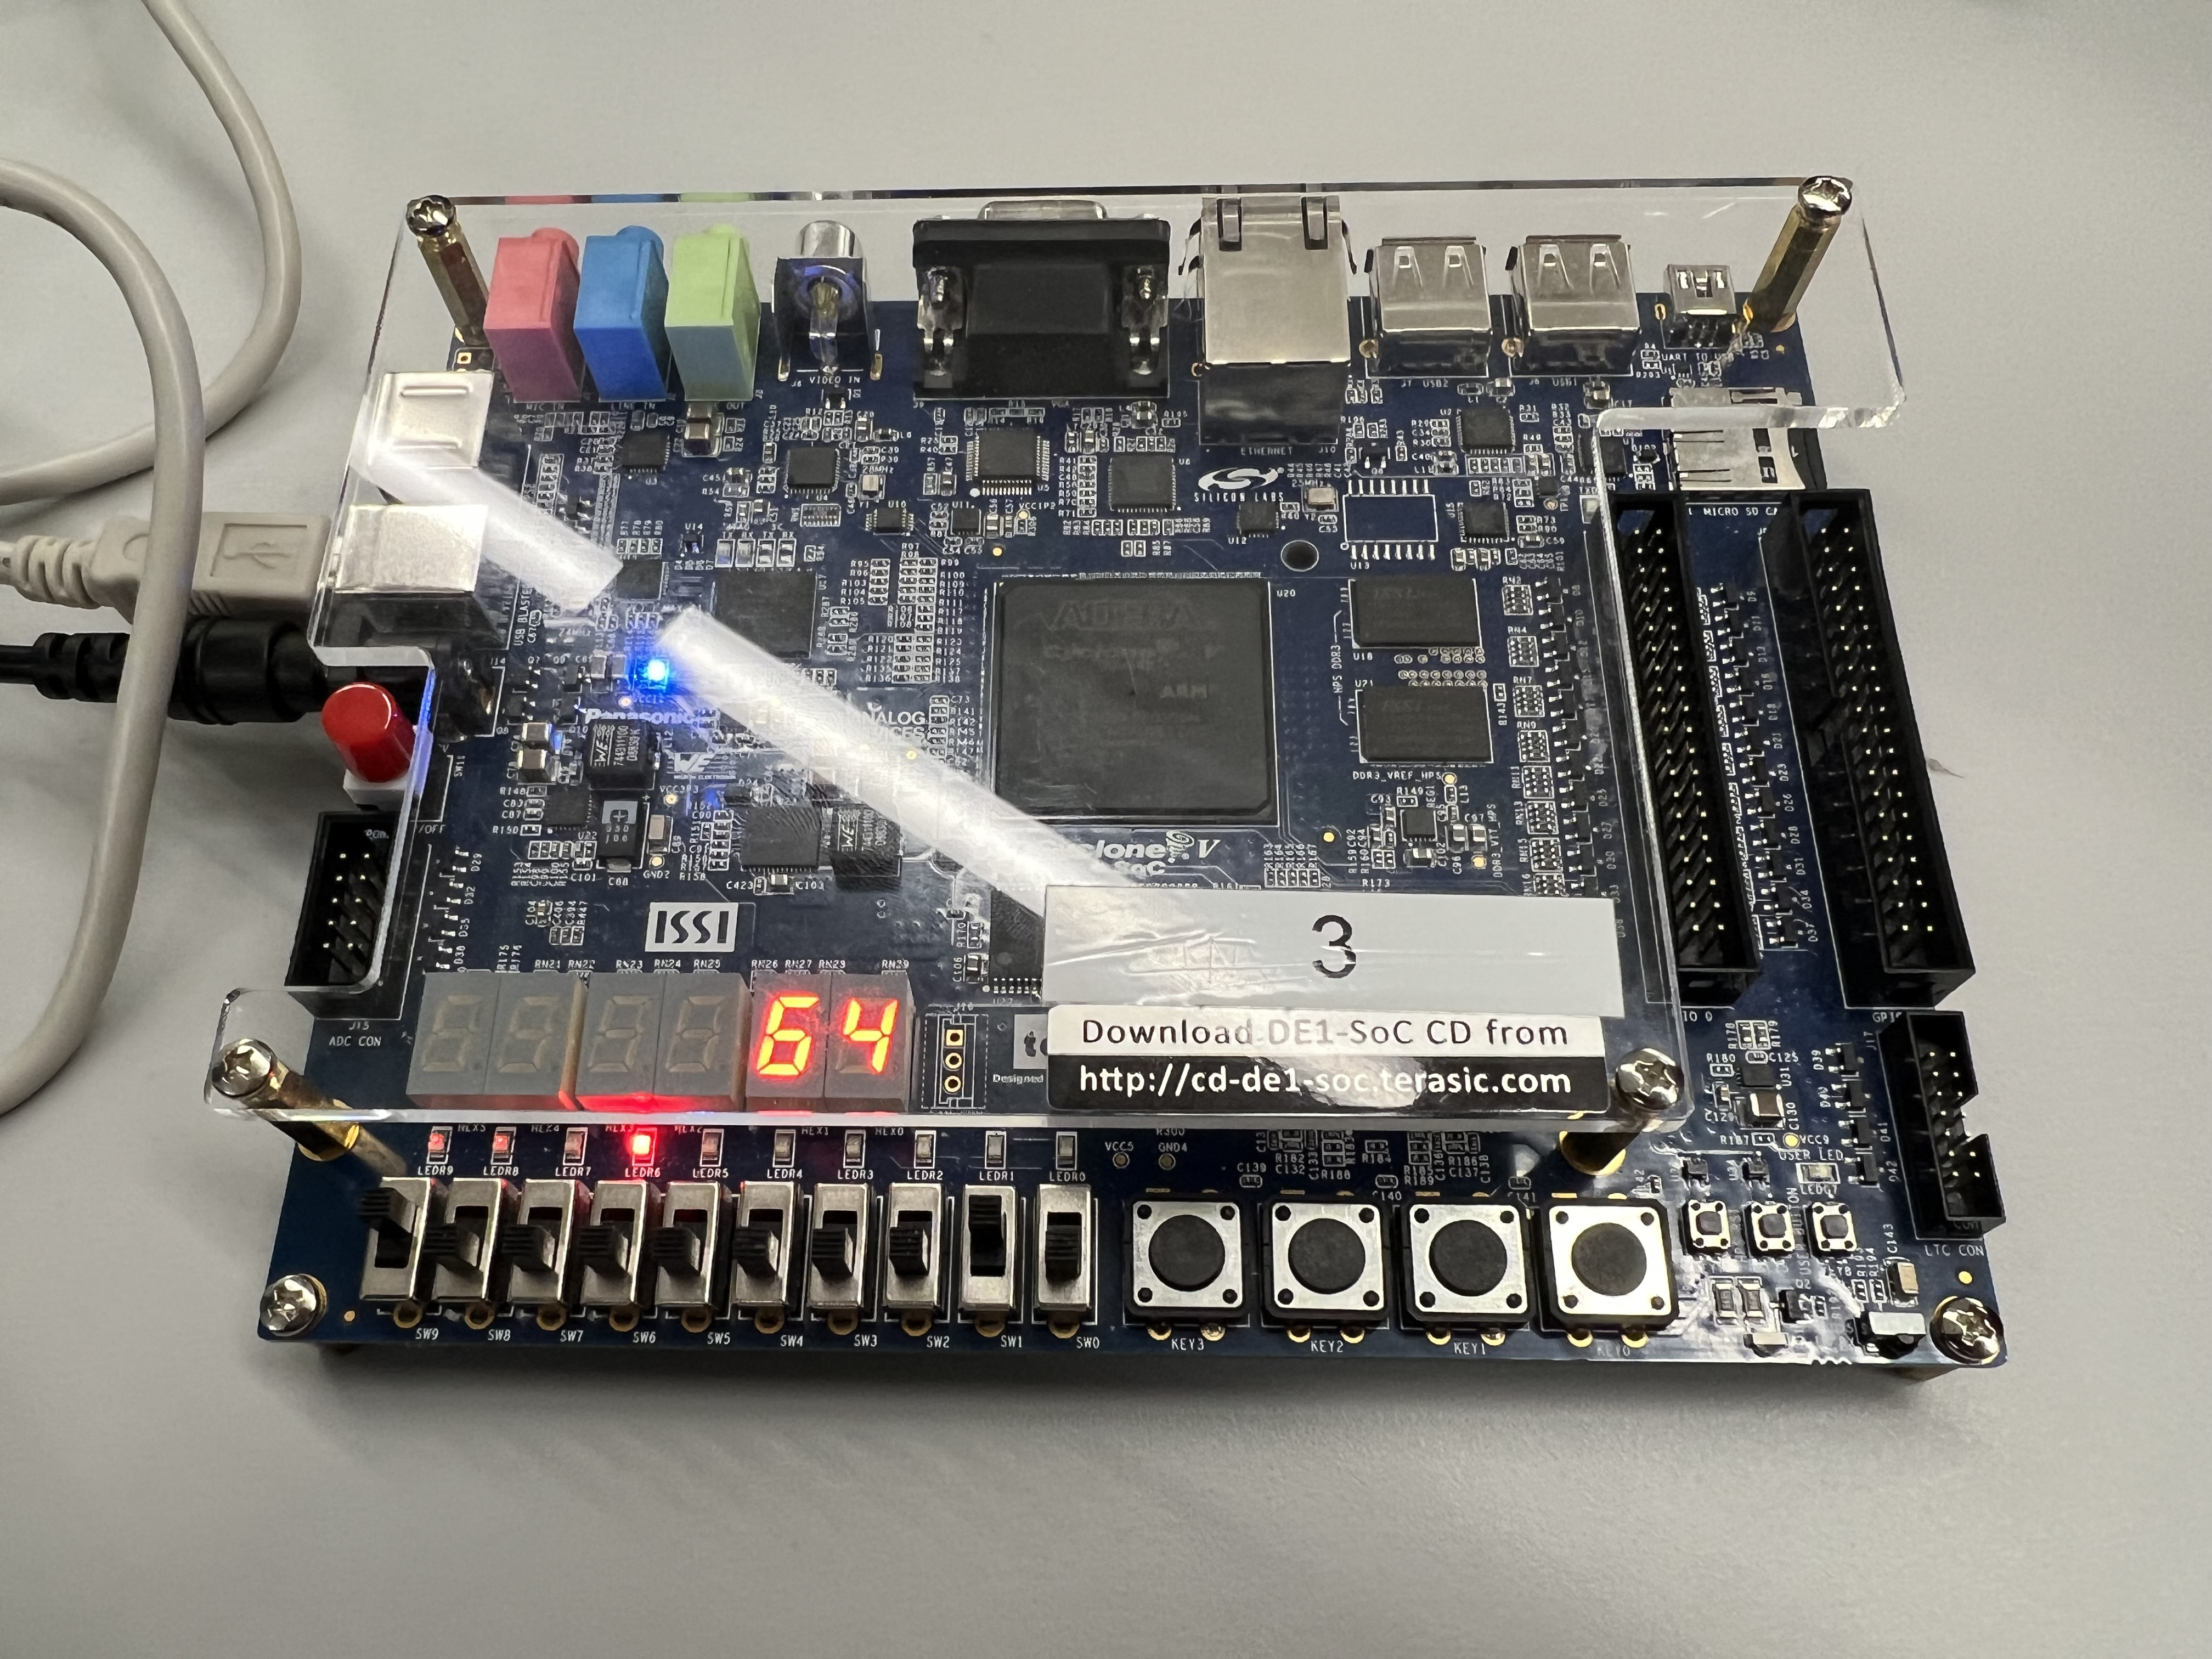
\includegraphics[width=.9\textwidth]{Figures/Part\ 2/IMG_1117.jpg}
  \caption{Multiplication — Binary Input of $00000010_2$ ($2$) and the Constant $32$}
  \label{fig:18}
\end{figure}

\section{Conclusion}

\hspace{.5 in} The lab resulted in the construction of two logical blocks: one that simply displayed an inputted binary number in decimal on the seven-segment displays, and another that performed arithmetic by using a control switch for a multiplexer, and then outputting to a seven-segment display, as well as binary LEDs. In this manner, an arithmetic logic unit (ALU) was constructed. Most importantly, the concepts of multiplexers was used for the first time, and allowed for an adequate introduction to multiplexers.

\end{document}
